\chapter{面向移动辅助机器人操控的柔性可穿戴体-机交互接口的自适应交互解码方法}
对于双侧上肢截肢患者和四肢瘫痪患者而言,定制化的人机交互界面在辅助机器人操控方面发挥至关重要的作用。高效的人机交互不仅仅可以提高他们的生活自理能力,且可以在一定程度上减轻社会和家庭的护理负担。在本章节中,研究基于柔性拉伸/弯曲传感器网络和一个惯性传感器设计了一种可穿戴式身体-机器交互界面。针对交互设备捕获肩部肌肉运动的感知数据,设计了两种数据映射模型:基于预定义规则的直接数据线性映射方式,以及考虑到肩部动作不确定性的意图推断数据解码方法。由于不同映射模式在动态响应能力以及精准度方面存在区别,研究通过一个实验将用户的使用直接数据映射模式的操作表现先验知识结合到共享自主方法中,实现了两种数据解码方式的自适应切换,进而增强数据解码在不同任务中的适应性。最后,研究通过一系列光标操控实验和虚拟电动轮椅驾驶任务验证了所提出交互界面和数据解码方法的有效性。

\section{研究动机与交互不确定性分析}    
四肢瘫痪和双侧上肢截肢对患者的生活质量造成极大影响,同时严重影响他们自我护理的能力。四肢瘫痪通常是由于脊髓较高位置的横贯性病变所导致,具体而言,位于第二胸椎以上的颈脊髓横贯性病变引发的截瘫,被称为高位截瘫。根据中国残疾人联合会数据,中国的肢体残疾人数量为2400万人左右,其中截肢和四肢瘫痪是肢体残疾中较为严重的类型之一,他们中的大多数人最终部分或完全依赖于他们的照顾者\cite{vitorinodinizRachimeduralTraumaEpidemiology2016}。世界卫生组织已经呼吁各国积极推进辅助设备的研究,我国在2021年九月发布了《中国脊髓损伤者生存质量白皮书》意在促进脊髓损伤辅助相关研究工作的推进。根据一项调查研究表明,除了恢复运动能力外,他们的主要兴趣之一是能够控制辅助机器人或电子设备,例如电脑、轮椅、机械臂和智能假肢。这些设备将有效提高他们日常生活的独立性,并减轻家庭的照顾负担    \cite{orejuela-zapataSelfHelpDevicesQuadriplegic2019}。然而,由于他们运动能力的缺陷,通常需要定制的人机交互界面来满足不同的需求。非侵入式的可穿戴人机交互接口通过实时跟踪身体某些部位的运动(如头部、手指、耳部肌肉等)来获取感知信号。由于这种接口侵入性较小,目前已有研究在探讨其作为定制化交互界面的潜力\cite{miehlbradtDatadrivenBodyMachine2018a,zhouNonInvasiveHumanMachineInterface2022}。与捕获脑机接口捕获大脑激活电信号不同,体机交互设备通常需要捕获人体的肌肉活动。因此,在设计定制化体-机交互界面之前,首先需要明确使用者的残余活动能力。颈椎脊髓损伤的分级主要依据ASIA(美国脊髓损伤协会)制定的标准\cite{SpinalCordInjury},具体如下:

\begin{figure}[htb]
    \centering
    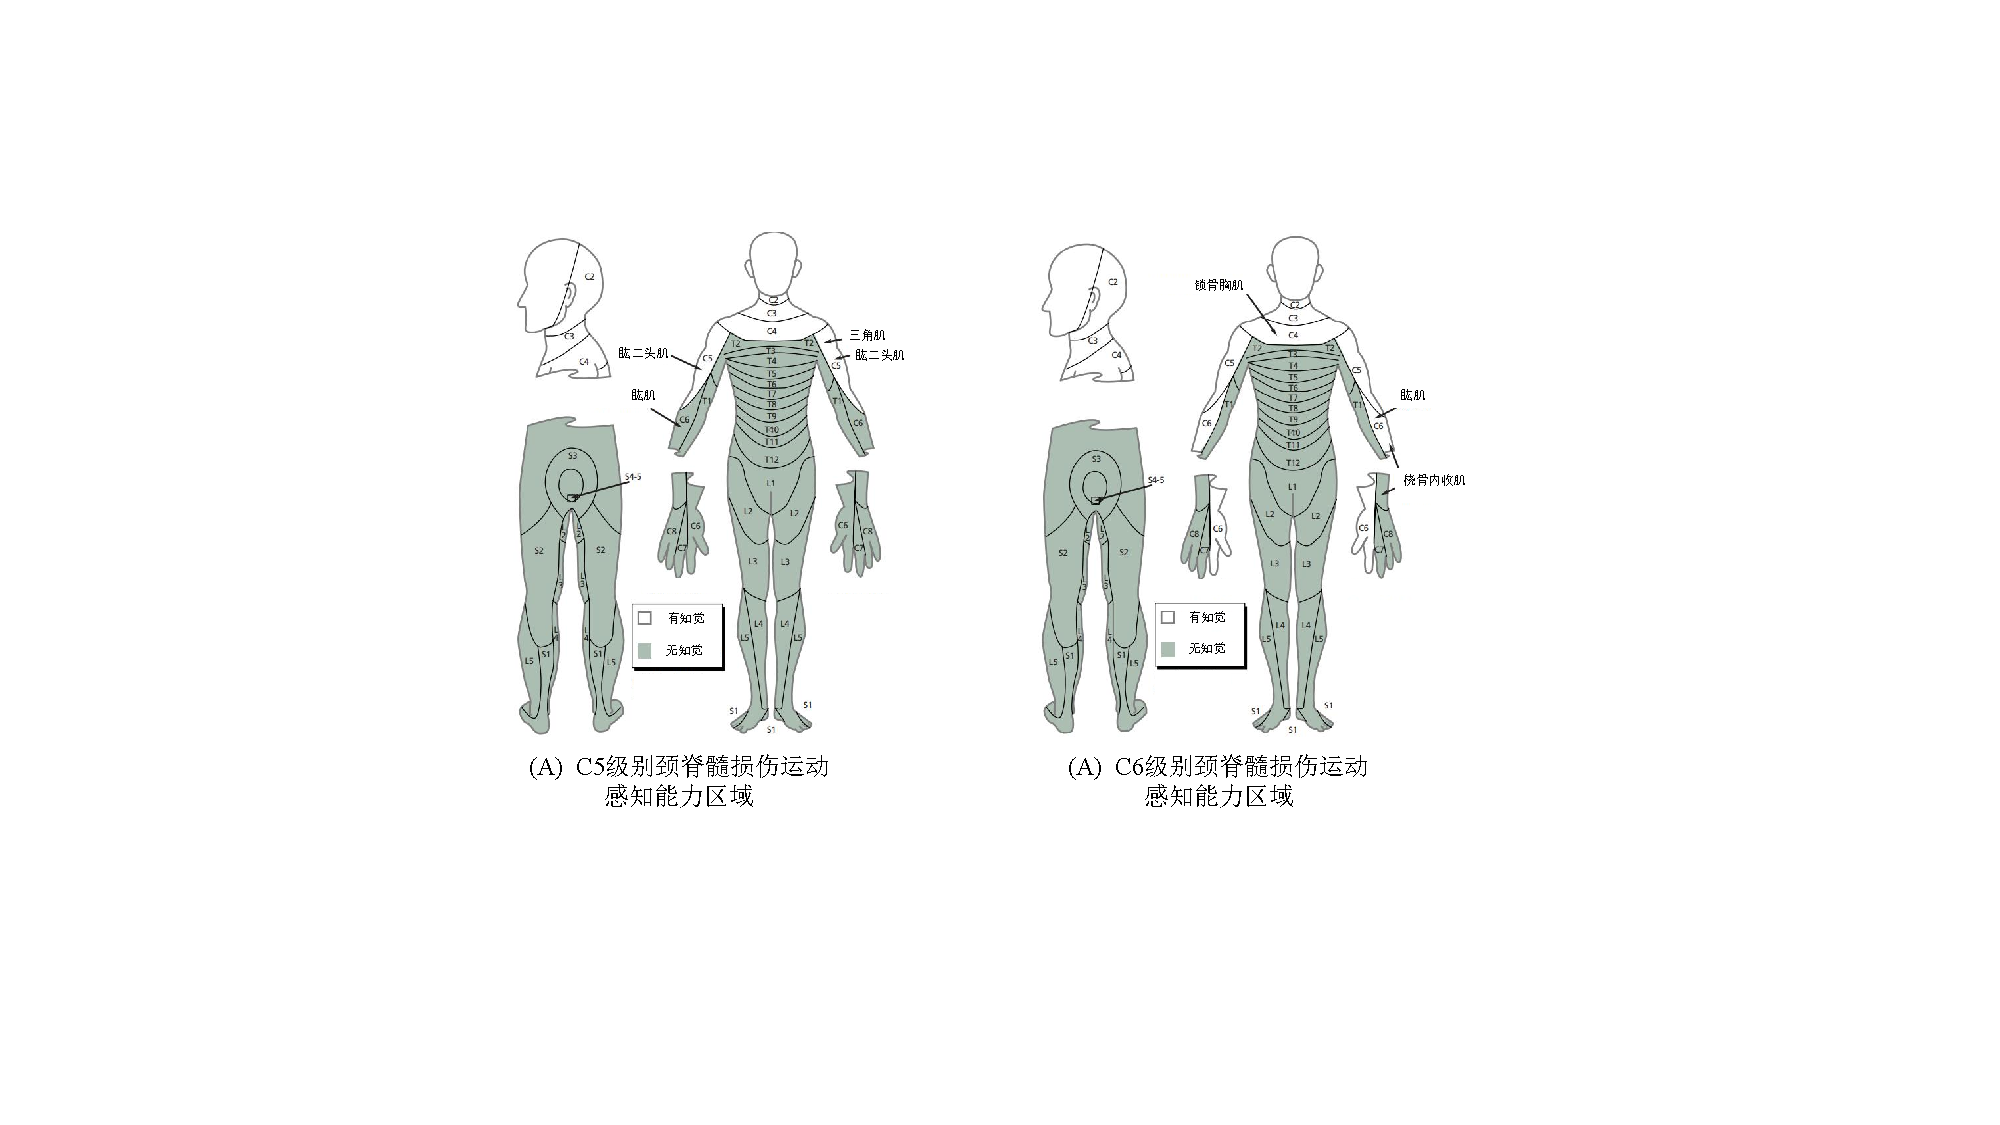
\includegraphics[width=1\textwidth]{3-Fig-1.pdf}
    \caption{C5与C6级别颈脊髓损伤全身运动感知能力分布示意图}
    \label{fig:3-1}
\end{figure}    

\begin{itemize}
\item A级:完全性脊髓损伤。损伤平面以下所有感觉、运动功能完全丧失,包括自主呼吸功能。患者需要终身依赖呼吸机或其他辅助设备维持生命。
\item B级:不完全性脊髓损伤。损伤平面以下存在感觉功能,但无运动功能。患者可以感知疼痛、温度等刺激,但不能进行自主运动。根据感觉功能保留的范围,B级又可分为B级-完全感觉和B级-部分感觉。
\item C级:不完全性脊髓损伤。损伤平面以下仅有一些肌肉运动的功能,无有用功能的存在。患者可以完成一些简单的动作,如移动肢体、维持姿势等,但无法进行日常生活活动或参与社会活动。
\item D级:不完全性脊髓损伤。损伤平面以下保留了部分的运动功能。患者可以完成一些日常生活活动,如行走、穿衣、进食等,但存在一定程度的障碍。根据运动功能保留的范围,D级又可分为D级-完全运动和D级-部分运动。
\item E级:正常或接近正常的脊髓功能。患者的感觉和运动功能基本正常,但可能存在一些异常的反射。这种情况通常不需要特殊治疗,患者可以恢复正常的生活和工作。
\end{itemize}

根据颈脊髓损伤的不同涉及节段,可将其分为C1至C8共8个级别,每个级别的症状均有所区别。C1至C4级别的颈脊髓损伤被视为高位损伤,其中C1和C2级别的损伤最为严重,常表现为颈部以下全身完全瘫痪、失去自主呼吸的能力、活动范围极为受限,患者需依赖护理人员进行全面照护,且因言语能力受损而导致沟通困难。对于完全无法进行自主活动的这类患者,由于他们无法使用任何辅助设备,本文不包含该情况的研究讨论。在C3和C4级别,患者有能力控制膈膜,因而可实现自主呼吸与言语交流。如图\ref{fig:3-1}所示,C5级别的患者则具备举起手臂或弯曲肘关节的能力,但可能无法控制手腕、手、躯干和双腿;尽管能说话,但呼吸能力有所衰减,可能需借助呼吸机,并需要帮助以清除体内积聚的唾液。这些患者可操作电动轮椅,但进出轮椅需要他人协助,同时需要借助特殊设备进食,每天需有2至6小时的人工帮助完成日常生活。C6级别患者在手腕伸展功能上受限,常在手部、躯干和腿部体验到麻痹感,但仍能向后弯曲手腕;他们能够说话,但呼吸功能较弱,自行上下床时不需要外部辅助。C7至C8级别的患者能控制某些手部动作,许多可以自行完成抓握与释放物品的操作,他们的言语能力正常,可以活动肩膀、手臂和手,但部分手部肌肉感觉减弱。综合来看,大多数不完全性脊髓损伤四肢瘫痪患者在其肩部周围仍有剩余的主动活动能力\cite{shefflerNeuromuscularElectricalStimulation2007},这为设计可穿戴体-机交互界面提供了可行性。

在第二章中,我们分析了闭环人机交互中控制外部设备的过程。使用体-机交互设备时存在三个主要的不确定性来源。(1)对用户当前状态观察不充分而存在的不确定性;(2)由于用户内部建立的环境动态模型与现实世界不匹配而导致的决策不确定性;(3)由于使用者身体机能限制导致的动作执行不确定性。(4)传感器的测量噪声。由于涉及多项不确定性来源导致难以分析,在本章研究中,我们首先假设用户对于环境的观测是充分的并且可以准确地获取环境状态,则可认为${o_t}{\text{ = }}{{\text{s}}_t}$。此外,随着时间的推移,使用者可以通过练习了解真实的世界动态$T({s_t}|{s_{t - 1}},{u_{t - 1}})$。因此,在本章研究中,我们认为不确定性只存在于使用者的动作和传感器的观测中,尽管柔性传感器测量中固有噪声相较于惯性传感器与生理信号传感器大大降低,但是体-机交互界面和用户身体在特定位置潜在的随机滑动仍然会导致不确定性的存在。其中人类动作的不确定性已被广泛研究\cite{churchlandCentralSourceMovement2006,vanbeersRoleExecutionNoise2004, desantisGuidingFunctionalReorganization2020a},相关研究报告了人类动作不确定性可以由高斯模型进行建模研究。因此,本章研究在建立意图推断模型时,将动作不确定性和传感器噪声合并建模为一个高斯分布,并将用户控制光标运动的状态转移不确定性同样也建模为高斯分布。

\section{柔性体-机交互接口系统设计} 

已有研究采用了惯性测量单元与视觉传感器来收集瘫痪患者的肩部活动数据,进而控制智能轮椅\cite{thorpUpperBodyBasedPower2016d,seanez-gonzalezCursorControlKalman2014}。然而,这些系统仅能测量所附着标记或传感器位置的移动,无法选择性地捕获用户的相应肌肉激活模式,容易受到外部环境噪声的干扰。为解决这一问题,已有研究将肌肉电信号与惯性传感器结合以捕获肌肉运动\cite{rizzoglioHybridBodyMachineInterface2020},但是该类型方法仍然需要捕获高质量的生理信号。可穿戴式的柔性应变传感器目前成为一种设计人机交互界面的一种新方法\cite{dongStretchableHumanMachine2020}。柔性传感器可以通过在不显眼的方式下测量皮肤或纺织品的形变来对人体运动进行跟踪。与惯性传感器不同,柔性传感器通常不存在积分漂移的问题,因此线性度以及可重复性较好,不需要频繁校准系统。当附着在特定肌肉群的位置时,柔性传感器可以通过测量肌肉的形变进而选择性地捕捉肌肉激活模式或关节运动信息。由于柔性传感器捕获的信息具有物理意义,因此相较于生理电信号通常更可靠且可以实现实时的计算处理。目前,柔性应变传感器已被部分研究用于捕捉人体肩关节的运动学信息\cite{jinSoftSensingShirt2020,leePrintableSkinAdhesive2016,samper-escuderoEfficientMultiaxialShoulderMotion2020}或设计实现上身/全身姿态的运动捕捉\cite{contreras-gonzalezEfficientUpperLimb2020,ogataEstimatingMovementsHuman2019,kimDeepFullBodyMotion2019}。目前,大多数相关研究都集中于使用传统的运动捕捉系统作为参考。他们通过采集大量人体运动学数据,并应用监督学习建立回归模型,进一步把柔性传感器的数据转换为关节角度。本章节与之前的研究有所不同。鉴于人体肩部是上肢中最为复杂的部分,研究首先分析肩部的骨骼肌肉模型,确定传感器的最佳位置,以便更有效的采集运动数据。此外, 本研究还设计了一套高效的数据解码方法,能够处理传感数据采集中的不确定性,将高维传感器数据转换成适用于不同任务的低维控制命令。

\subsection{人体肩部肌肉骨骼模型}
肩关节是人体活动度最大同时也是最不稳定的关节。它能进行多种运动:在额状面可以做屈伸,在矢状面可以做外展和内收,在水平面可以环绕和屈伸,而在垂直方向可以内旋和外旋。从骨骼结构看,肩部由肩胛骨、锁骨和肱骨组成;肩胛骨是这一区域最大的骨骼,并在后背位置与锁骨和肱骨共同构成了肩关节;锁骨位于胸部上方,连接着肩胛骨和肱骨,让手臂获得了活动自如的能力;肱骨则为手臂的主骨,贯通肩关节至肘关节,使手臂能够弯曲和伸直。肩部的肌肉可分为四组:(1)肩胛肌:主要控制肩胛骨,包括斜方肌、菱形肌、抬肩胛肌和前锯肌。(2)只跨越肩关节的肌肉:如三角肌、喙肱肌、二头肌和三头肌。(3)跨越两个以上关节的肌肉:这类肌肉有胸大肌和背阔肌。(4)与肩功能间接相关但重要的肌肉:如冈上肌、冈下肌和小圆肌。这些肌肉与韧带一同工作,协助完成抬举手和旋转肩膀等复杂运动\cite{terryFunctionalAnatomyShoulder2000}。

\begin{figure}[htb]
    \centering
    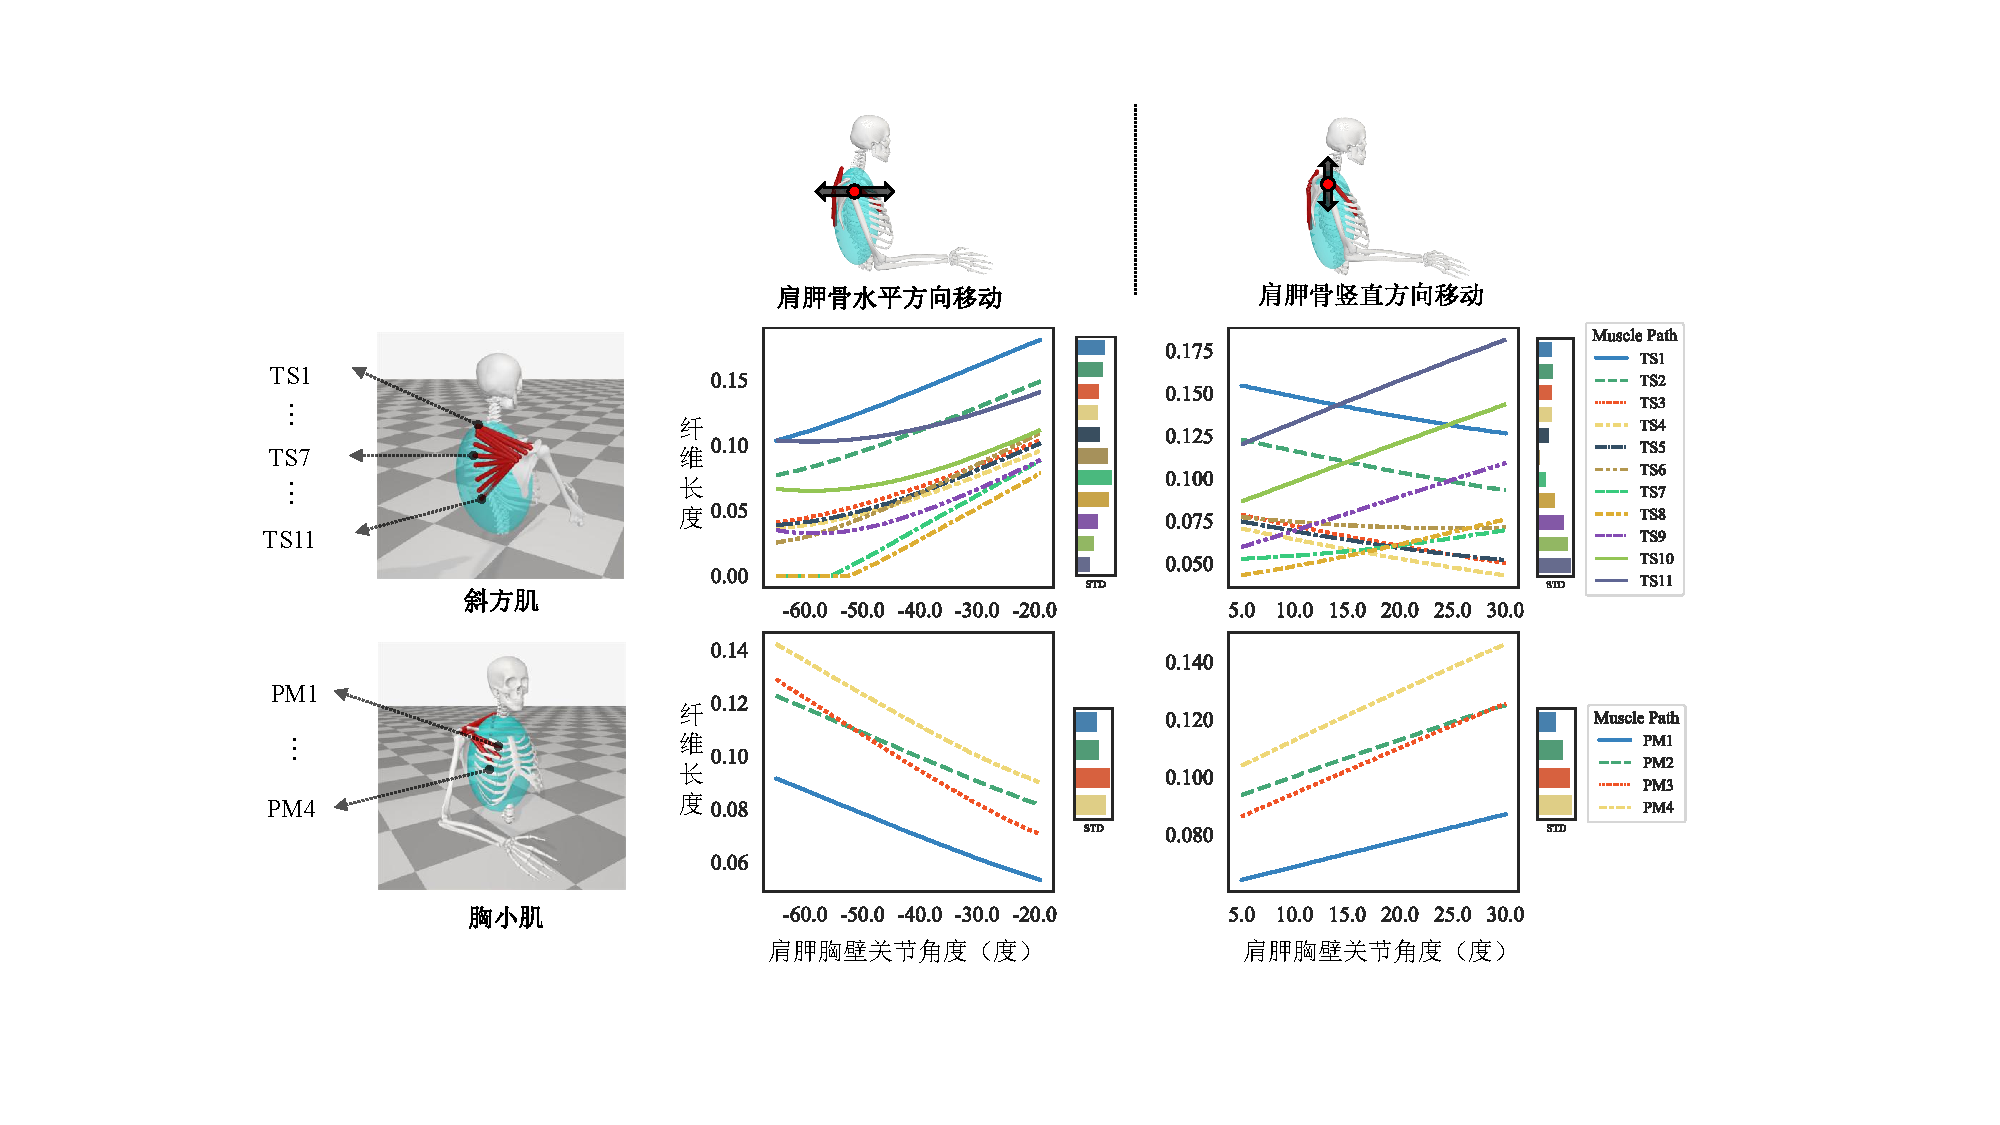
\includegraphics[width=0.9\textwidth]{3-Fig-2.pdf}
    \caption{斜方肌和胸小肌群肌肉纤维标准化长度随肩胛胸壁关节运动的变化,其中条形图显示了每组肌肉纤维随肩部运动变化的肌肉形变量标准偏差}
    \label{fig:3-2}
\end{figure}

所设计的交互设备通过捕获肩胛骨运动(或称肩胛胸壁关节的运动)以生成连续命令,而不是依赖肩关节角度。肩胛骨参与上升、下降、前伸、后缩、上旋和下旋等六种类型的活动自由度。由于活动范围较小无法产生足够的肌肉形变,研究在骨骼肌肉模型的分析中省略了上旋和下旋两种运动模式。这些动作主要负责上肢的升降,需要大范围的运动,不适合四肢瘫痪的人。如图\ref*{fig:3-2}所示,基于OpenSim\cite{chadwickRealTimeSimulationThreeDimensional2014}的肩关节肌肉骨骼模型仿真,首先对斜方肌和胸小肌在水平和竖直两个方向上运动的肌纤维标准化长度变化特征进行了研究。斜方肌参与肩胛骨的后缩,促使肩胛骨向脊柱方向移动,反之,胸小肌对肩胛骨施加向下的力,使其向胸部移动。在肩胛骨水平前伸和后缩过程中,斜方肌和胸小肌的标准化肌纤维长度呈现出相反的变化趋势。值得一提的是,在垂直肩胛运动过程中,斜方肌的肌肉路径TS7至TS11展现出与胸小肌路径中观察到的类似变化趋势。鉴于此,研究制定了两项柔性传感器放置准则,以便最大限度地扩增所涉及交互设备可捕获的肌肉运动动态范围。首先,所选的肌肉路径在相同的运动范围内应表现出最大的标准偏差。其次,斜方肌和胸小肌的标准化长度变化应在肩胛关节运动的同一方向上呈现出相反的趋势。

\subsection{交互系统硬件设计}如图\ref{fig:3-3}所示,所开发的交互系统重量为430克,通过聚合物锂离子电池供电,在运行时的功耗约为270mW。该系统使用了四个单轴柔性弯曲/拉伸传感器和两个双轴弯曲硅胶数字电容式柔性应变传感器(由美国Nitto Bend Technologies公司生产),各个柔性传感器通过FPC排线连接至数据同步模块,并通过I2C总线以50Hz的速率将所采集到的数据上报。单轴柔性传感器能够捕获一个方向上解耦的路径无关弯曲和拉伸位移信息,而双轴柔性传感器则可以捕获两个正交方向上的路径无关弯曲信息。为了降低传感器与身体之间的滑动对于测量精度的影响,在设计中于压缩衬衫内放置了硅胶防滑带,并通过3D打印外壳将软传感器固定于衬衫上。根据上一节所提出的传感器放置准则,我们将四个单轴软传感器(L1、L3、R1、R3)被放置在肌肉路径TS7、TS8、TS9和PM3、PM4区域,用于捕捉相应肌肉的活动。两个双轴软传感器(L2、R2)安装在肌肉路径TS1、TS2、TS3区域,用于捕获水平和垂直方向的肩部活动。

\begin{figure}[htb]
    \centering
    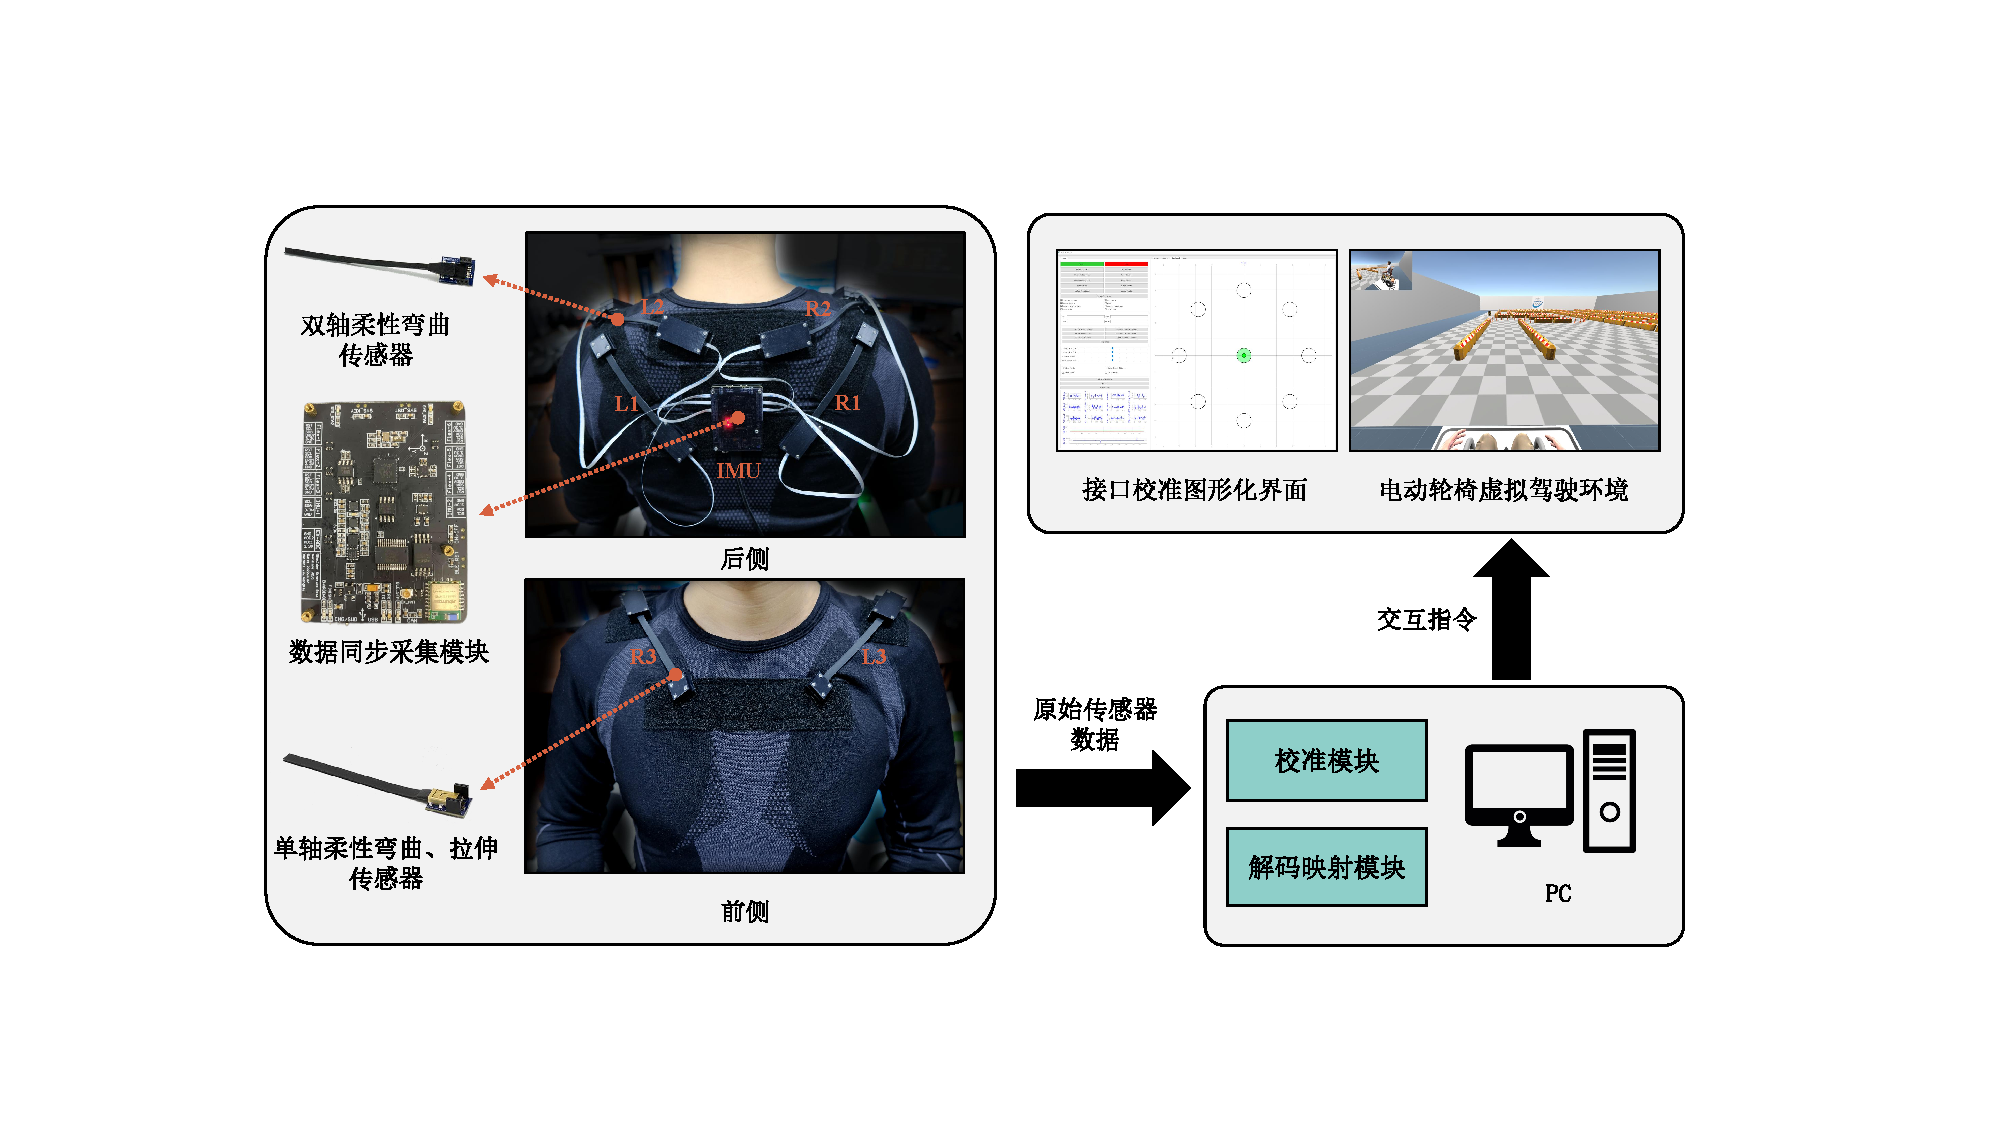
\includegraphics[width=0.8\textwidth]{3-Fig-3.pdf}
    \caption{所设计的体-机交互界面硬件系统结构以及相应的柔性传感器布置位置}
    \label{fig:3-3}
\end{figure}     

数据同步模块置于用户背部中央区域,图\ref{fig:3-4}给出了该模块的结构框图。本模块利用STM32F103 MCU进行开发,并集成了UCOS III操作系统以实现任务的调度。模块的PCB板上集成了一个MEMS惯性传感器MPU6050,其中包含三轴加速度计和三轴陀螺仪,并且通过I2C中继器与柔性传感器进行通信。数据同步采集模块能够以50Hz的频率将传感器数据同步上传至上位机(配备Intel i5 10400F 2.9Ghz的计算机),通过无线蓝牙和有线USB两种方式进行。此外,模块采用了一个分辨率为$3840\times2160$的27英寸显示器,放置在用户前方60厘米的位置,用以提供视觉反馈。上位机的图形界面用于辅助校准和提供任务指导。

\begin{figure}[htb]
    \centering
    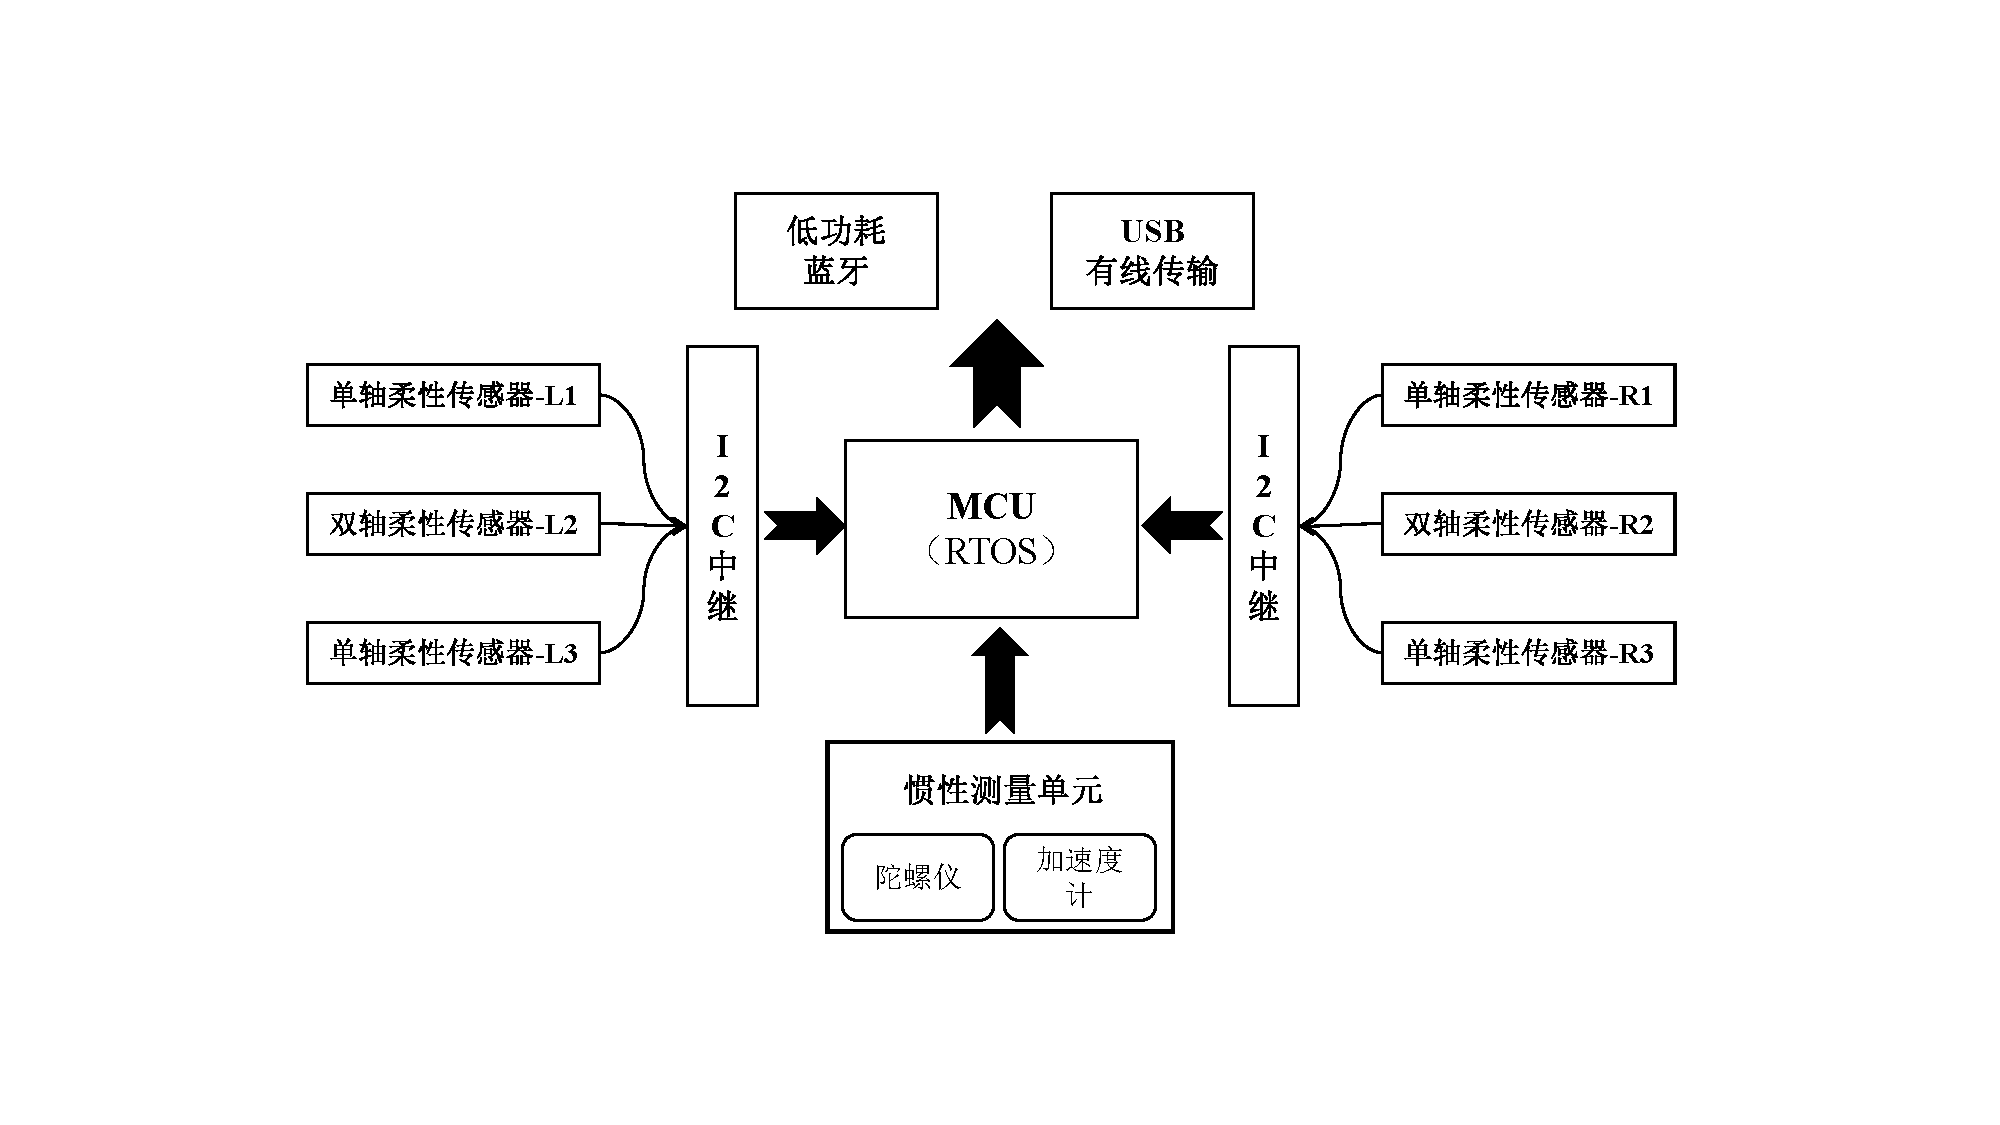
\includegraphics[width=0.8\textwidth]{3-Fig-4.pdf}
    \caption{数据同步采集模块的硬件系统结构框图}
    \label{fig:3-4}
\end{figure} 
\section{传感器数据处理与解码} 
受Gopinath等人对于防止使用者意外交互界面操作的研究\cite{gopinathCustomizedHandlingUnintended2021}的启发,我们认为预期操作$a_t$与结果操作之间的偏差是不可忽略的。对于运动障碍人士来说,固有的身体限制会增加出现动作偏差的可能性。根据用户意图提供命令至关重要,而不是仅仅依赖于传感系统的测量值,因此研究开发了两种方法分别实现了映射函数$m(y_t)$将观测信息解码为操控指令。  

\subsection{基于确定性规则映射的数据解码}
将数据从传感系统直接映射到命令空间代表了一类端到端人机交互解码方法,其中传感器信号直接通过一个线性或非线性的映射函数实现命令生成,无需考虑系统中存在的不确定性因素。图\ref{fig:3-5}的给出了基于确定性规则映射的数据解码方法的概率图模型,其中${y_t}$是在每个时间步长获得的传感系统的观测值。${{p}_t} = m({{y}_t})$是由一个线性函数$m$映射的控制命令。

\begin{figure}[htb]
    \centering
    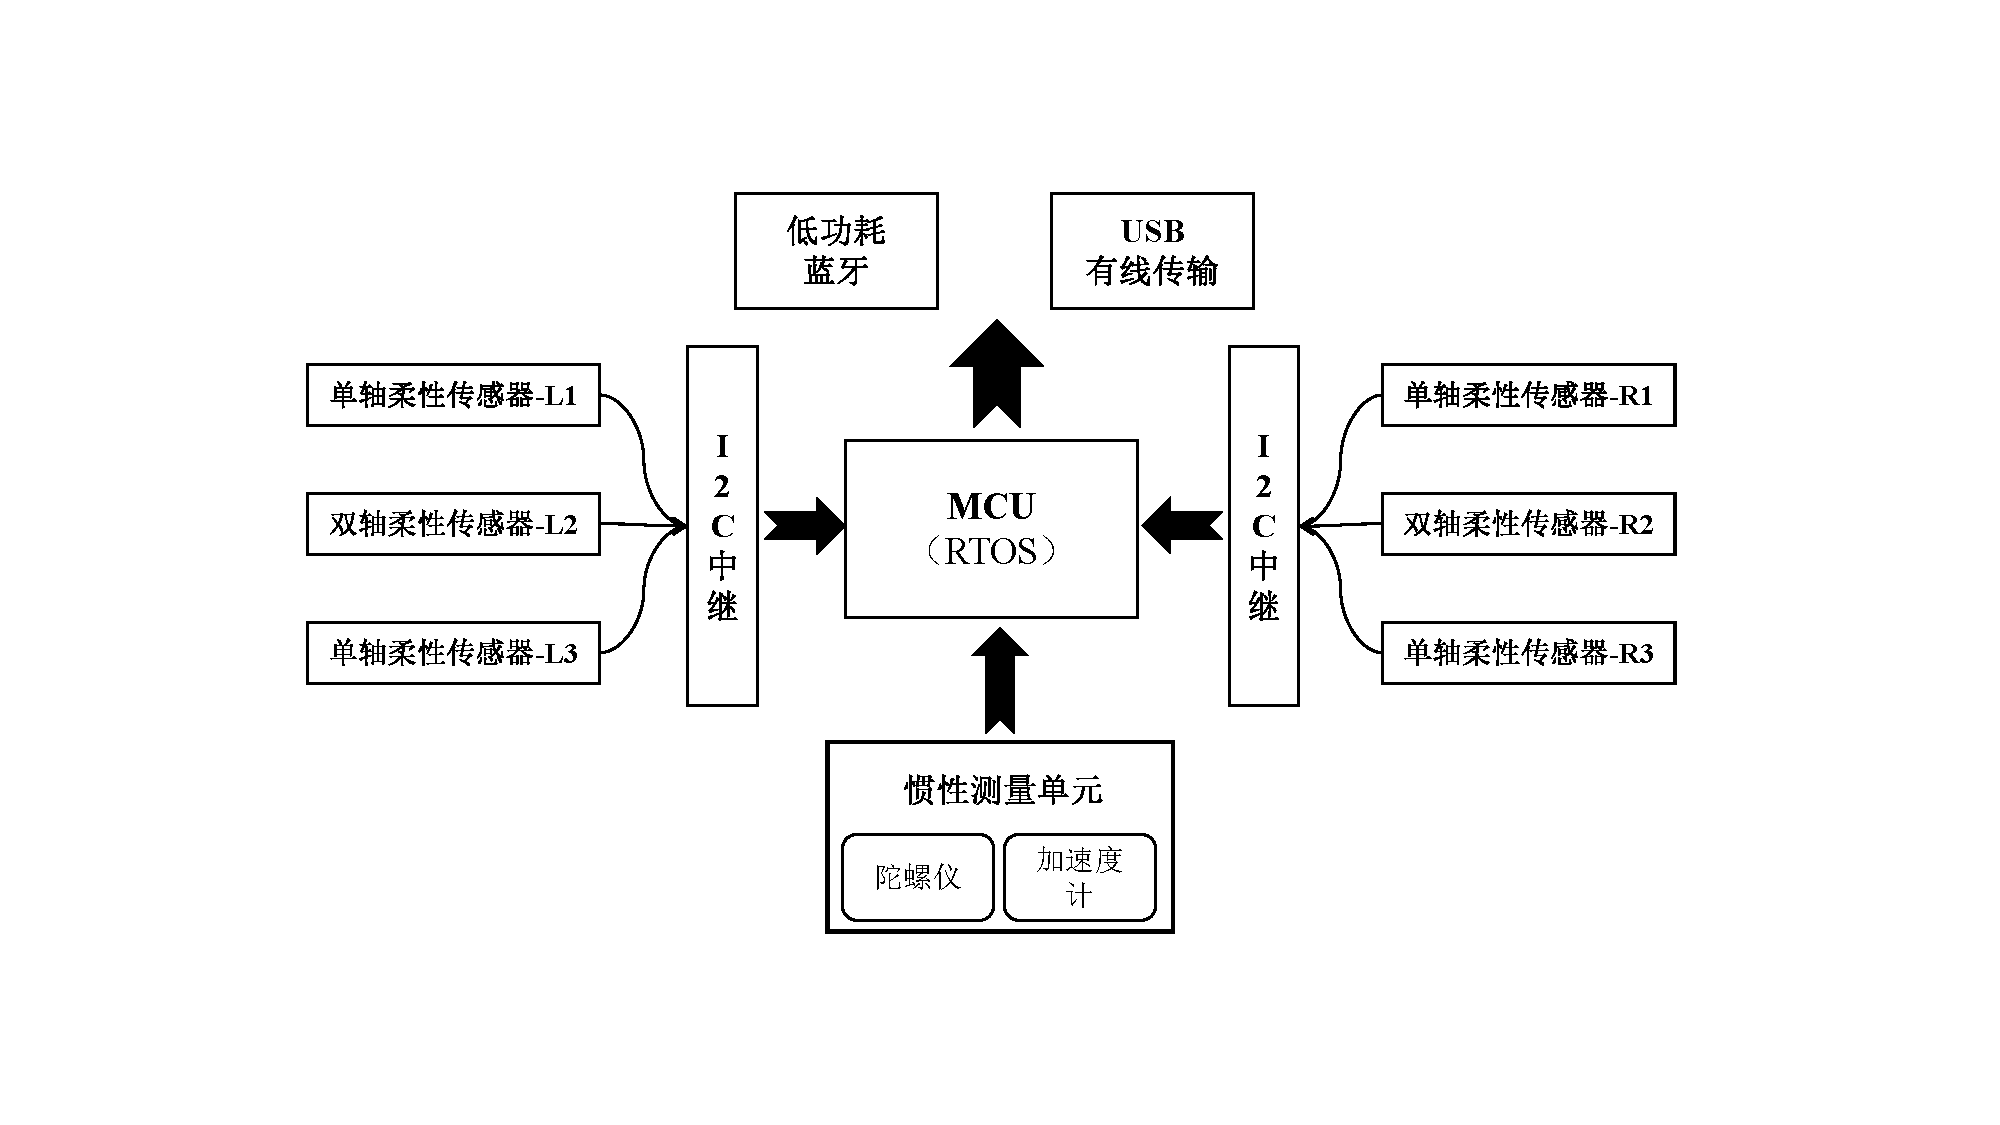
\includegraphics[width=0.8\textwidth]{3-Fig-5.pdf}
    \caption{基于确定性规则映射的数据解码方法的概率图模型以及肩部动作与光标动作之间的关系}
    \label{fig:3-5}
\end{figure} 

\subsubsection{映射规则设计}
在相关研究中,主成分分析(PCA)方法通常用于将体-机交互界面的高维数据映射到低维操作命令\cite{casadioBodyMachineInterface2011,seanez-gonzalezStaticDynamicDecoding2017}。然而,基于PCA的映射模型对于用户来说往往难以将其和自身运动建立起一个清晰和直观的关系(例如光标移动方向和身体运动趋势不一致),导致用户需要大量的时间才能熟练使用它。为了解决这个问题,如图\ref{fig:3-6}所示,研究设计了一种基于规则的数据映射解码方式,将高维水平肩部运动映射到二维命令空间。其中,肩胛胸壁关节进行前伸运动生成的命令位于象限 \uppercase\expandafter{\romannumeral1}、\uppercase\expandafter{\romannumeral2}内,肩部后缩运动生成的命令位于象限\uppercase\expandafter{\romannumeral3}、\uppercase\expandafter{\romannumeral4}内。低维度的映射函数输出向量${p_t}$和操控命令输出$u_t^{DCM}$的计算方式如下

\begin{equation}
{p_t} = {\kern 1pt} \mathbf{{F}} \cdot \mathbf{{P}} \cdot {y_t}
\label{eq1}
\end{equation}   

\begin{equation}
\label{eq2}
u_t^{DCM} \triangleq {G_d}\left( {{p_t} - C_z} \right) \odot C_a
\end{equation}   

其中在$t$时刻的观测${y_t} = {[y_t^{(L1)},y_t^{(L3)},y_t^{(R1)},y_t^{(R3)}]^T}$是柔性传感器L1、L3、R1和R3测量的拉伸位移形变量。常数${G_d}$用于调整生成的命令的增益,$C_b\in {\mathbb{R}^{2 \times 1}}$和$c \in {\mathbb{R}^{2 \times 1}}$分别代表了零位置校准向量和尺度缩放校准向量,这两个向量在校准程序中获得。矩阵$\mathbf{P} \in {\mathbb{R}^{4 \times 2}}$是映射规则矩阵,$\mathbf{F} \in {\mathbb{R}^{2 \times 2}}$是单位旋转矩阵,它将$p_t$逆时针旋转$\pi /4$。最后,研究将左侧或右侧放置在胸小肌和斜方肌的两个柔性应变传感器的观测值之差作为命令,因此可以得到基于确定性规则的观测映射矩阵:

\[{\mathbf{F}} \cdot {\mathbf{P}} = \frac{{\sqrt 2 }}{2}\left[ {\begin{array}{*{20}{c}}
{\begin{array}{*{20}{c}}
1&{ - 1}  \\  
1&1 
\end{array}}&{\begin{array}{*{20}{c}}
{ - 1}&1  \\  
{ - 1}&{ - 1} 
\end{array}} 
\end{array}} \right]\]   

\subsubsection{校准过程}
基于确定性规则映射的数据解码的校准环节包括两个阶段。首先,在实验中我们要求参与者佩戴者以舒适放松的姿势静坐10秒钟,记录所用软传感器的拉伸数据,然后按照下式计算零点校准向量$C_b$:

\begin{equation}
C_b = \frac{1}{T}{\left[ {\sum\nolimits_{i = 1}^T {{g^x_i}} ,\sum\nolimits_{i = 1}^T {{g^y_i}} } \right]^T}
\label{eq3}
\end{equation}    

其中$T$是在10秒内记录数据的数量,${g^x_t}{\text{ = }}y_t^{({\text{L}}1)} - y_t^{({\text{L}}3)}$、${g^y_t}{\text{ = }}y_t^{({\text{R}}1)} - y_t^{({\text{R}}3)}$分别是使用者左肩和右肩位于胸小肌和斜方肌柔性传感器拉伸形变量的差值。在校准过程的第二阶段,参与者被要求尽可能最大幅度重复地前后移动肩膀10秒,在后期数据处理中通过使用峰值检测算法捕获记录的校准数据的极值点,用于计算缩放校准向量$C_a = {[{s_x},{s_y}]^T}$,其中${s_x}$和${s_y}$是缩放因子,计算公式为

\begin{equation}
{s_x} = \left \{  \begin{gathered}
    \frac{{\sum\nolimits_{i = 1}^{T_x^ + } {X_i^ + } }}{{T_x^ + }},{g^x_t} > 0 \hfill  \\ 
    \frac{{\sum\nolimits_{i = 1}^{T_x^ - } {X_i^ - } }}{{T_x^ - }},{g^x_t} < 0 \hfill  \\  
  \end{gathered}  \right.{\text{, }}{s_y} = \left \{\begin{gathered}
    \frac{{\sum\nolimits_{i = 1}^{T_y^ + } {Y_i^ + } }}{{T_y^ + }},{g^y_t} > 0 \hfill  \\ 
    \frac{{\sum\nolimits_{i = 1}^{T_y^ - } {Y_i^ - } }}{{T_y^ - }},{g^y_t} < 0 \hfill  \\  
  \end{gathered}  \right.
  \label{eq4}
\end{equation}

其中$X_i^ + ,X_i^ - $和$Y_i^ + ,Y_i^ - $分别是第二阶段校准数据中的正峰值和负峰值。完成校准环节后,使用者自由使用身体探索光标的控制,并且手动调整它们认为最佳的增益$G_d$。

\subsection{基于状态估计意图推理的交互不确定性处理方法}基于规则的直接映射数据解码未考虑系统的不确定性因素,根据前述分析,这一做法是有缺陷的。因而,研究进一步在体-机交互设备的解码过程中考虑使用者的肩部交互动作不确定性,并将其引入系统分析。在这一框架下,用户意图所产生的交互指令被视为不可观测的隐状态。

\begin{figure}[htb]
    \centering
    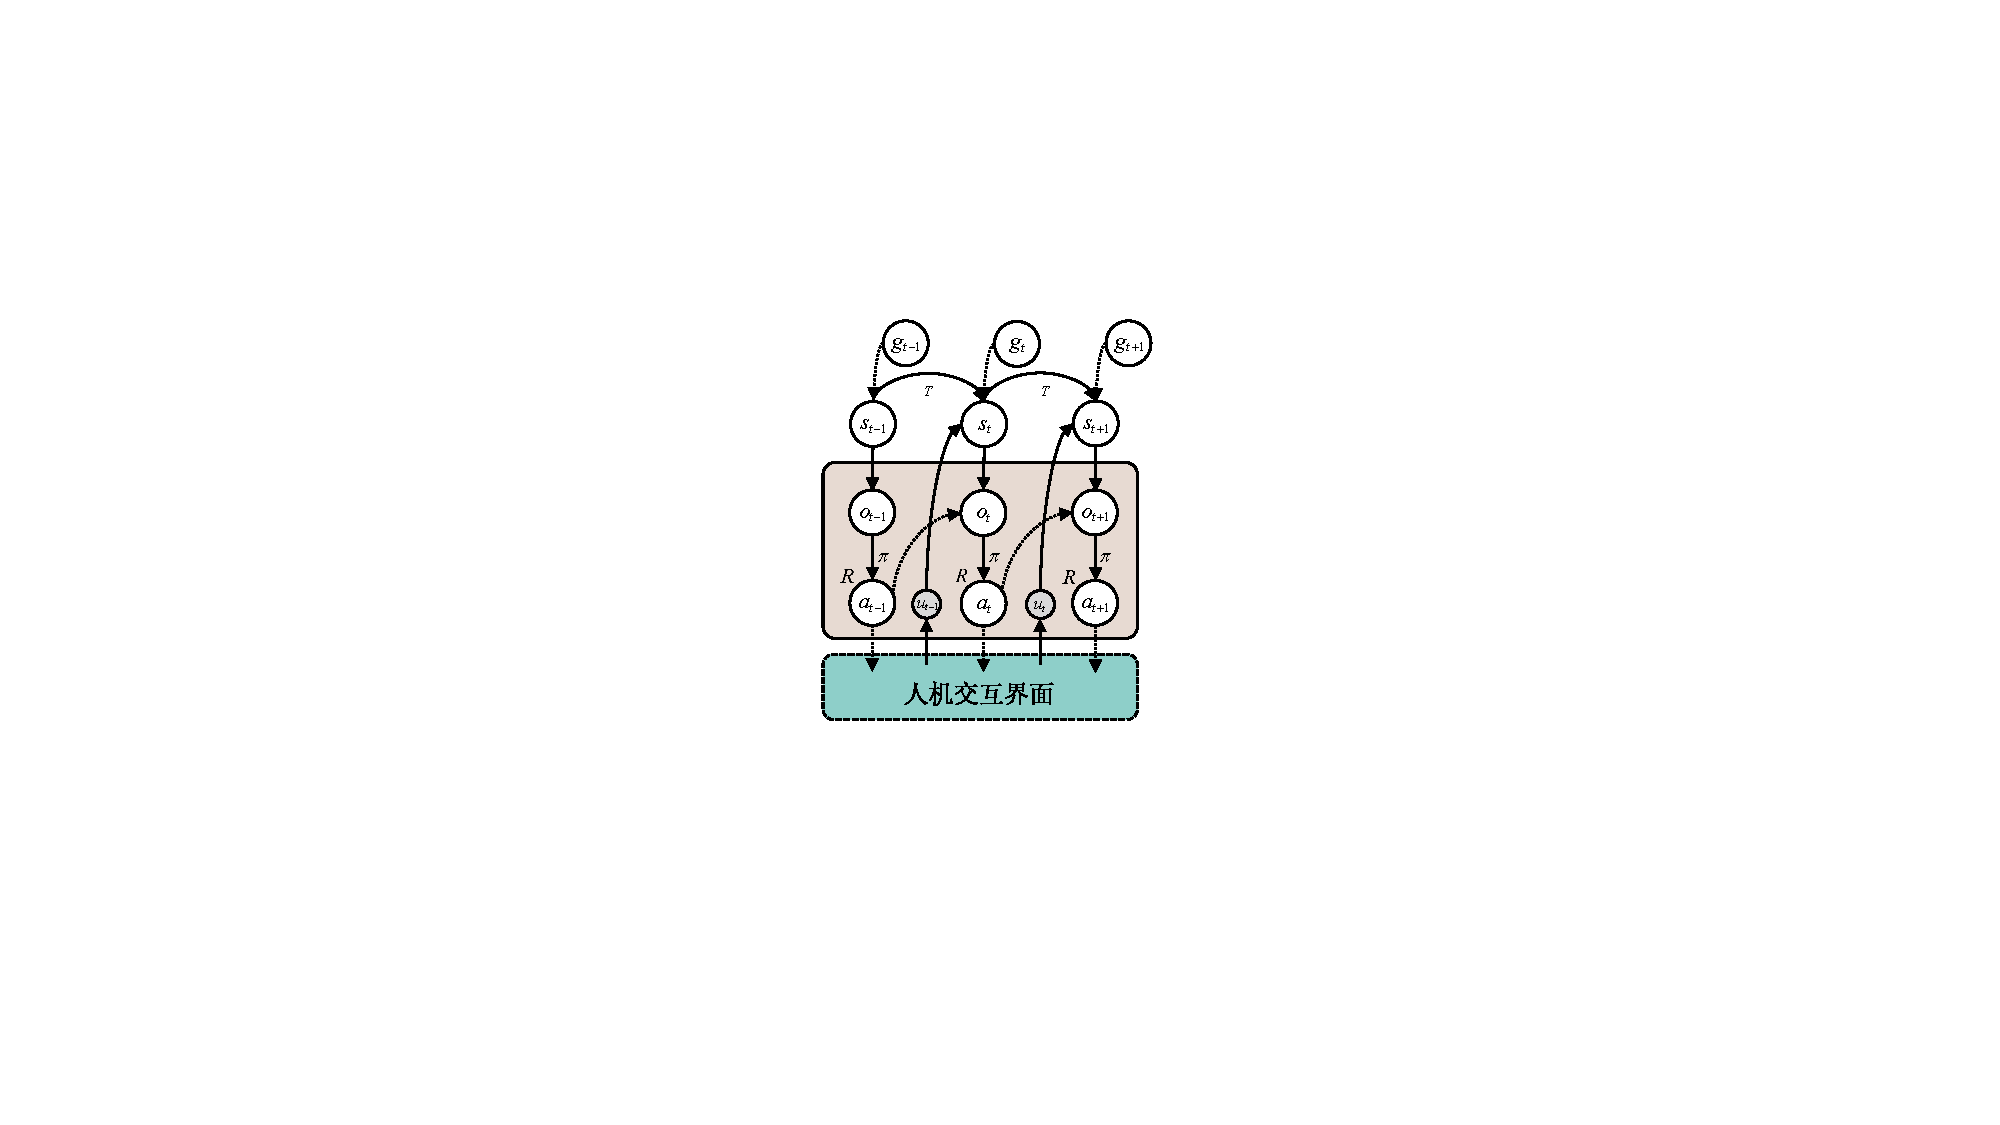
\includegraphics[width=0.4\textwidth]{3-Fig-6.pdf}
    \caption{基于意图推理的数据解码方法的概率图模型}
    \label{fig:3-6}
\end{figure}

\subsubsection{意图推理的概率模型}
图\ref{fig:3-8}给出了基于意图推理的数据解码方式的概率图模型给出,相较于基于规则的数据映射,其在${a_t}$和${y_t}$之间添加了不可观测的潜在变量${z_t} \in \Phi $用于表示使用者的意图,其中$\Phi$是潜在命令空间,用于表示用户可能期望发出的所有命令,在本任务中被定义为一个连续的二维平面中的位置。具体而言,${z_t}$ 代表了用户基于对当前状态和目标的认知所期望产生的指令。在时间点 $t$,潜在用户意图 ${\hat z_t}$ 的推断依赖于后验概率 $p({z_t}|{y_{1:t}})$ 的期望值,其中 $y_{1:t} \in {\mathbb{R}^{t \times N}}$ 是累积的体-机交互接口的观测数据,$N$ 是用于推断的传感器的数据维度。由于在设计当中使用了多组柔性传感器以及一个惯性传感器,其信息往往是冗余的,需要选择使用。由于我们无法直接建立观测到意图的映射关系,因此其由一个消融实验来确定。
\begin{equation}
    \label{eq5}
    \hat z_t = \mathop{argmax}_{z_t} p({z_t}|{y_{1:t}})
\end{equation}
经过校准后的输出指令 $u_t^{UII}$ 的定义为:
\begin{equation}
\label{eq6}
u_t^{UII} \triangleq {G_i} \cdot {\hat z_t}
\end{equation}    
其中$G_i$是比例因子,在校准阶段由使用者手动调整。为了简化计算,研究进一步假设了用户的在$t$时刻意图的操控命令与$t+1$时刻的命令之间的关系是线性的,此外假设观测数据到意图之间的映射函数$f(y_t)$也是线性的。其中相邻两个时刻的意图指令之间和传感器测量与当前意图指令之间的不确定性是服从高斯分布的,当其满足马尔科夫齐次性假设和观测独立性假设时,该模型可以表示为:

\begin{equation}
\label{eq7}
p({z_t}|{z_{t - 1}}) = \mathcal{N}({\mathbf{A}}{z_{t - 1}},{{\mathbf{Q}}})
\end{equation}   

\begin{equation}
\label{eq8}
p({y_t}|{z_t}) = \mathcal{N}({\mathbf{C}}{z_t},{{\mathbf{R}}})
\end{equation}    

其中$p({z_t}|{z_{t - 1}})$为状态转移条件概率,$p({y_t}|{z_t})$为观测条件概率。${z_t} = [{p_x}(t),{p_y}(t),{v_x}(t),{v_y}(t)]$是使用者潜在命令在时间$t$的状态,在本任务中具体表现为一个在二维空间中移动的点(光标)。${\mathbf{A}} \in {\mathbb{R}^{4 \times 4}}$是连续时间步之间潜在命令的先验动力学状态转移矩阵,${\mathbf{C}} \in {\mathbb{R}^{N \times 4}}$是传感器观测与当前用户意图命令之间的观测矩阵。${{\mathbf{Q}}} \in {\mathbb{R}^{4 \times 4}}$和${{\mathbf{R}}} \in {\mathbb{R}^{N \times N}}$分别表示了使用者的潜在意图命令在进行状态转移时的不确定性以及交互界面观测的不确定性。基于以上假设,对于使用者的意图推理过程可以看作一个状态估计问题,其最优估计可以通过卡尔曼滤波框架进行求解。研究将状态转移动力学矩阵${\mathbf{A}}$定义为:

\begin{equation}
\mathbf{A} = 
\begin{bmatrix}{}
1&0&{\Delta t}&0  \\  
0&1&0&{\Delta t}  \\  
0&0&1&0  \\  
0&0&0&1 
\end{bmatrix}
\end{equation} 

其中$\Delta t$是离散系统的时间步长,观测矩阵${\mathbf{C}}$和状态转移不确定性协方差矩阵${{\mathbf{Q}}}$以及观测不确定性协方差矩阵${{\mathbf{R}}}$以及可以根据意图推理校准环节采集得到的训练数据计算得出。


\subsubsection{概率模型的参数估计}基于意图推理的数据解码方首先需要通过一组运动想象任务进行数据采集,该任务目前通常被用于 脑机接口神经解码数据采集的过程\cite{malikEfficientDecodingSteadyState2011,brandmanRapidCalibrationIntracortical2018},近年来已应用于体-机交互界面数据解码\cite{seanez-gonzalezCursorControlKalman2014,seanez-gonzalezStaticDynamicDecoding2017}。在训练过程中,我们要求受试对象跟随一个在屏幕上直径为0.8厘米的红色指引光标,该光标在任务空间中沿着一条10厘米的直线从屏幕中心按照逆时针的顺序朝着八个方向移动。其中该红色光标的移动根据式\ref{eq3-9}所定义的微分方程进行移动\cite{seanez-gonzalezStaticDynamicDecoding2017},$tar_x(t)$和$tar_y(t)$分别代表了光标在显示器上的二维平面中的位置,$[tar_x(0),tar_y(0)]$和$[tar_x(f),tar_y(f)]$分别为光标的起点和终点位置,$\tau$为时间常数用于控制光标的运动速度。运动想象任务是开环的,这意味着在实验中我们不会向用户提供当前其当前使用交互界面生成的命令的任何反馈信息。受试对象需要完成三次独立的数据采集任务,期间记录红色目标光标移动的数据(位置和速度)和体机交互界面所采集的传感器原始数据。

\begin{equation}
    \begin{aligned}
    & tar_x(t)=tar_x(0)+\left(tar_x(0)-tar_x(f)\right)\left(15 \tau^4-6 \tau^5-10 \tau^3\right) \\
    & tar_y(t)= tar_y(0))+\left(tar_y(0))- tar_y(f))\right)\left(15 \tau^4-6 \tau^5-10 \tau^3\right)
    \end{aligned}
    \label{eq3-9}
\end{equation}

观测矩阵${\mathbf{C}}$通过运动想象务中所采集的训练数据的最大似然估计来获得,计算方式如下:

\begin{equation}
    \mathbf{C} = YX^T(XX^T)^{-1}
\end{equation}
状态转移不确定性协方差矩阵${{\mathbf{Q}}}$和表示观测不确定性的协方差矩阵${{\mathbf{R}}}$可以通过类似的方法计算得到,计算方法如下:
\begin{equation}
{\mathbf{Q}} = \frac{1}{N_D-1}(X_2 - AX_1)(X_2 - AX_1)^T
\end{equation}

\begin{equation}
{\mathbf{R}} = \frac{1}{N_D}(Y - CX)(Y - CX)^T
\end{equation}
其中,$Y$是由运动想象任务记录的体-机交互界面的传感器测量和$X$矩阵为数据采集过程中相应的屏幕中的指引光标位置数据组成的。数据矩阵$X_1\triangleq X_{1:end-1}$和$X_2\triangleq X_{2:end-1}$,$N_D$为采集的训练数据量。

完成运动想象训练的数据采集和参数更新后,使用者可以通过在任务空间中自由地移动控制光标控件来手动调整增益${G_i}$。当用户感觉当前训练的意图推理模型不能很好地工作时,实验将数据采集和训练重新进行直至使用者可以使用他们的肩胛骨控制光标运动。至于用于意图推理的传感器信息数$N$的确定,将通过一个消融实验深入研究。  

\subsection{基于共享自主的自适应命令映射解码切换}  基于确定性规则映射的数据解码方式仅依靠当前时刻的传感器观测值,因此可以进行高效率的命令生成。另一方面,基于意图推理的数据解码方式通常需要累积更多的观测数据作为``证据''进而推理出交互意图,虽然其考虑了交互过程中的不确定性使得估计产生的命令更加精确,但是其同时会导致交互界面生成命令的动态性能下降。如果想要提高交互界面的动态性能,则系统中将不可避免地引入更多不确定性。虽然使用者可以利用视觉或其他反馈进行调整,但这会在一定程度上增加使用者的认知负荷。另一方面,意图推理通过对不确定噪声的过滤,会导致交互界面生成指令的带宽下降进而导致用户在需要快速响应控制的情况下由于反馈延迟下意识地增加其动作的幅度导致无法实现对辅助设备稳定的控制,在相关研究\cite{seanez-gonzalezStaticDynamicDecoding2017}中也报告了类似的问题。

\begin{figure}[htb]
    \centering
    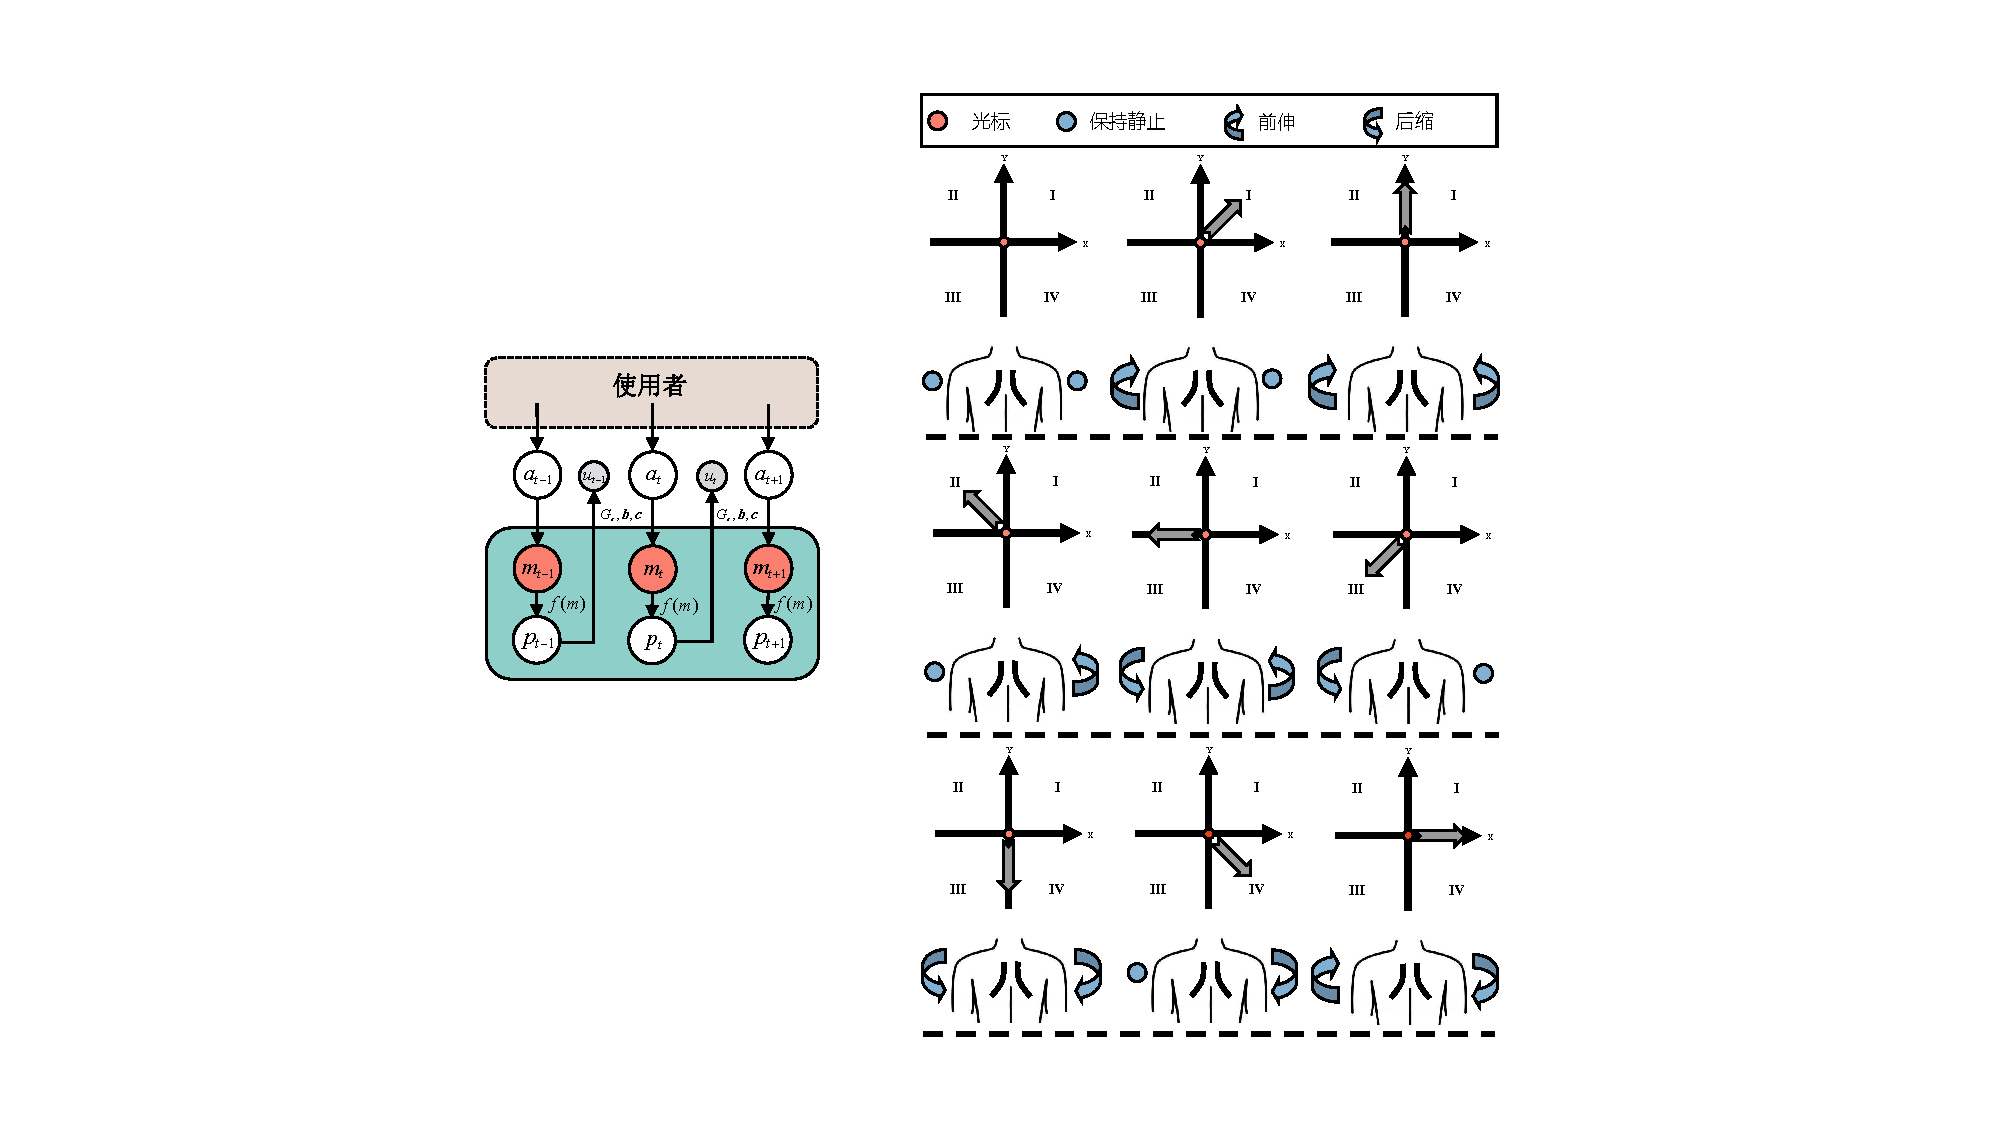
\includegraphics[width=1\textwidth]{3-Fig-7.pdf}
    \caption{基于共享自主的自适应命令映射解码方法的概率图模型}
    \label{fig:3-7}
\end{figure} 

\subsubsection{仲裁函数定义} 
通过将共享自主系统引入交互界面的解码过程,研究认为以基于确定性规则的数据解码方式为主的命令生成方式,辅以意图推理的自适应介入辅助可以实现操作指令在高动态性能表现下的同时提高其指令的准确性。为了实现解码方式的自适应切换,在该工作中通过将个性化先验知识嵌入到一个仲裁函数中来实现推理的自适应介入。图\ref{fig:3-7}给出了基于共享自主的自适应命令映射解码的概率图模型,其中用户的动作可以由基于确定性规则的数据解码(虚线)和基于意图推理的数据解码同时处理,并通过一个非线性仲裁函数实现自适应切换。特别地,由于所设计体-机交互界面在每个时刻都观察到${y_t}$,因此我们可以认为存在条件独立关系${z_t} \bot {p_t}|{y_t}$。共享数据解码方法输出的命令$u_t^{SCM}$定义为:
\begin{equation}
    \label{ex6}
    u_t^{SCM}\triangleq \lambda_{\mathcal{F}} u_t^{UII}+(1-\lambda_{\mathcal{F}})u_t^{DCM}
\end{equation}   

其中$\lambda_{\mathcal{F}}  \in [0,1]$是用于仲裁从两种数据映射解码方式的混合系数,共享自主系统的混合因子由预训练用户能力模型$\mathcal{F}(u)$动态调整。为了保证解码方式切换的平滑性,研究将其定义为一系列局部线性模型的加权线性组合,该方法也被称为感受野加权回归模型\cite{schaalScalableTechniquesNonparametric2002},定义如下式:
\begin{equation}
    \label{ex7}
    \mathcal{F} (u) \triangleq \frac{{\sum\nolimits_{i = 1}^K {{w_i}{g_i}(\hat u)} }}{{\sum\nolimits_{k = 1}^K {{w_i}} }}{\text{,  }}{g_i}(\hat u) = {\theta}_i^T{\hat u}
\end{equation}

公式中$\hat u = {[\begin{array}{*{20}{c}}{{u^T}}&1\end{array}]^T}$,其中${u} = u_t^{SCM}\in {\mathbb{R}^2}$是用户解码后二维命令空间中的位置向量,$K$是局部模型的数量,${g_i}(u)$是由${\boldsymbol{\theta }}_i^T \in {\mathbb{R}^{3}}$参数化的一阶线性多项式。权重${w_i\in {\mathbb{R}}}$根据一个径向基核函数计算:
\begin{equation}
    \label{ex8}
    {w_i} = \exp \left( { - 0.5 \times {{(u - {{c}_k})}^T}{{r}}(u - {c_k})} \right)
\end{equation}

其中$c_i \in \mathbb{R}$是径向基核函数的中心位置,参数$r$用于调整每个线性局部模型的感受野。每个局部模型的${\theta }_k$的参数可以通过实验中获得训练数据进行递归最小二乘得到。由于用户的表现会随着使用时间的增加而改变或提高,因此基于递归的优化允许通过增量学习的方式来更新模型。时间$t$处的混合因子的值定义为一个分段函数:
\begin{equation}
    \label{ex9}
    {\lambda _t} = \left \{{\begin{array}{*{20}{c}}
        {\begin{array}{*{20}{c}}
        0  \\  
        {\mathcal{F} (u)}  \\  
        1 
      \end{array}}&{\begin{array}{*{20}{c}}
        {,\mathcal{F} (u) < 0}  \\  
        {,0 < \mathcal{F} (u) < 1}  \\  
        {,\mathcal{F} (u) > 1} 
      \end{array}} 
      \end{array}} \right.
\end{equation}

\subsubsection{用户能力先验模型的建立}建立用户能力模型先验模型$\mathcal{F}(u)$的目的是希望明确使用者在命令空间中不同区域使用确定性映射规则进行指令生成的能力。然而,我们只能通过有限数量的实验来测试用户在不同命令空间位置的使用表现,因此在实验中我们设计了一个目标跟踪任务中用于量化的用户的操作表现。由于本任务中所设计的命令空间为一个连续的二维平面,若要通过实验得到用户能力的量化表征,首先需要对命令空间进行离散化。
\begin{figure}[htb]
    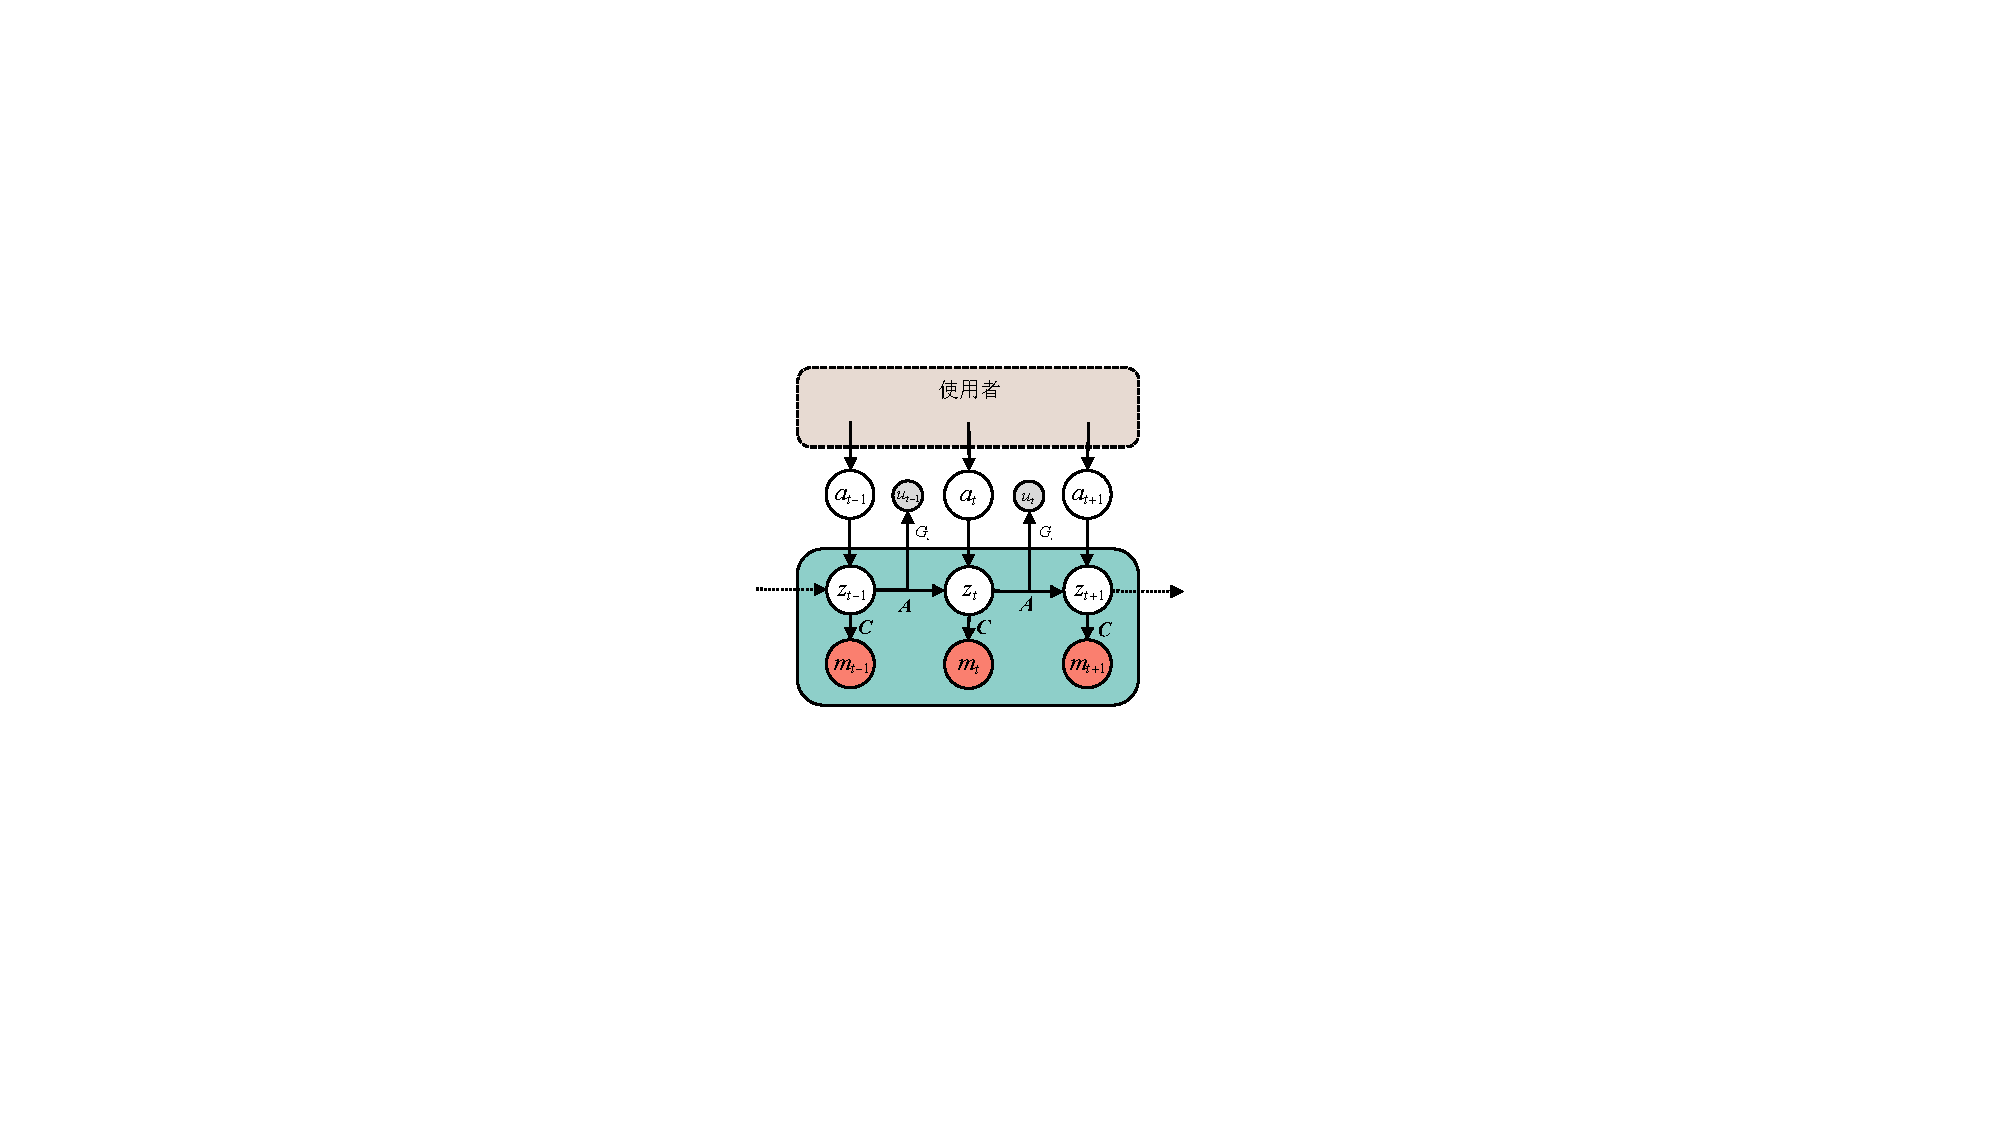
\includegraphics[width=1\textwidth]{figures/3-Fig-8.pdf}
    \caption{区域目标跟踪任务流程示意图}
    \label{fig:3-8}
\end{figure}

根据菲茨定律\cite{tangFittsLawModulated2018},将光标移动至目标中心的时间,受到目标大小和光标与目标间距离的影响。通过保持目标的大小以及传输时间和相邻目标之间的距离恒定。研究通过受试者控制的光标与高亮标记的区域中心之间的欧氏距离度量来定义受试者使用基于确定性规则映射的数据解码方式的能力。如图\ref{fig:3-8}所示,该区域目标跟踪任务涉及记录在命令空间中的一个 0.8 厘米的受控光标和屏幕上一个$1\times1$cm大小的蓝色高亮方形目标之间的距离值。目标在$20\times20$cm任务空间内(对应一个$5\times5$命令空间)以1秒的时间间隔以蛇形模式移动,参与者尽可能地使用肩部控制光标准确地跟踪高亮区域并保持光标在目标的指定区域内,在显示器上通过显示一个受控的蓝点光标提供实时视觉反馈,其中光标的位置$s$与目标$g$中心之间的欧几里德距离是在高亮方形目标开始转移到下一个位置时计算的,因此在一轮实验中将产生400个数据点。

\begin{equation}
    \label{ex12}
    d \triangleq \frac{1}{1+e^{-8\sqrt{(g-s)^T(g-s)}+4}} 
\end{equation}    
此处,$d$为一个非线性Logistic函数,其将偏移欧式距离度量的结果限制在0到1的范围内来量化用户的表现。在实验中,我们要求每名参与者完成三次任务,最终将得到每次实验命令空间中与目标位置$g_c$相关的1200组数据$[g_c,d]$。先验模型$\mathcal{F}(u)$由25个线性模型$g_k(\hat u)$组成,其中每个线性局部模型的中心$c_k$以2的间隔均匀分布在命令空间中。
\begin{figure}[htb]
    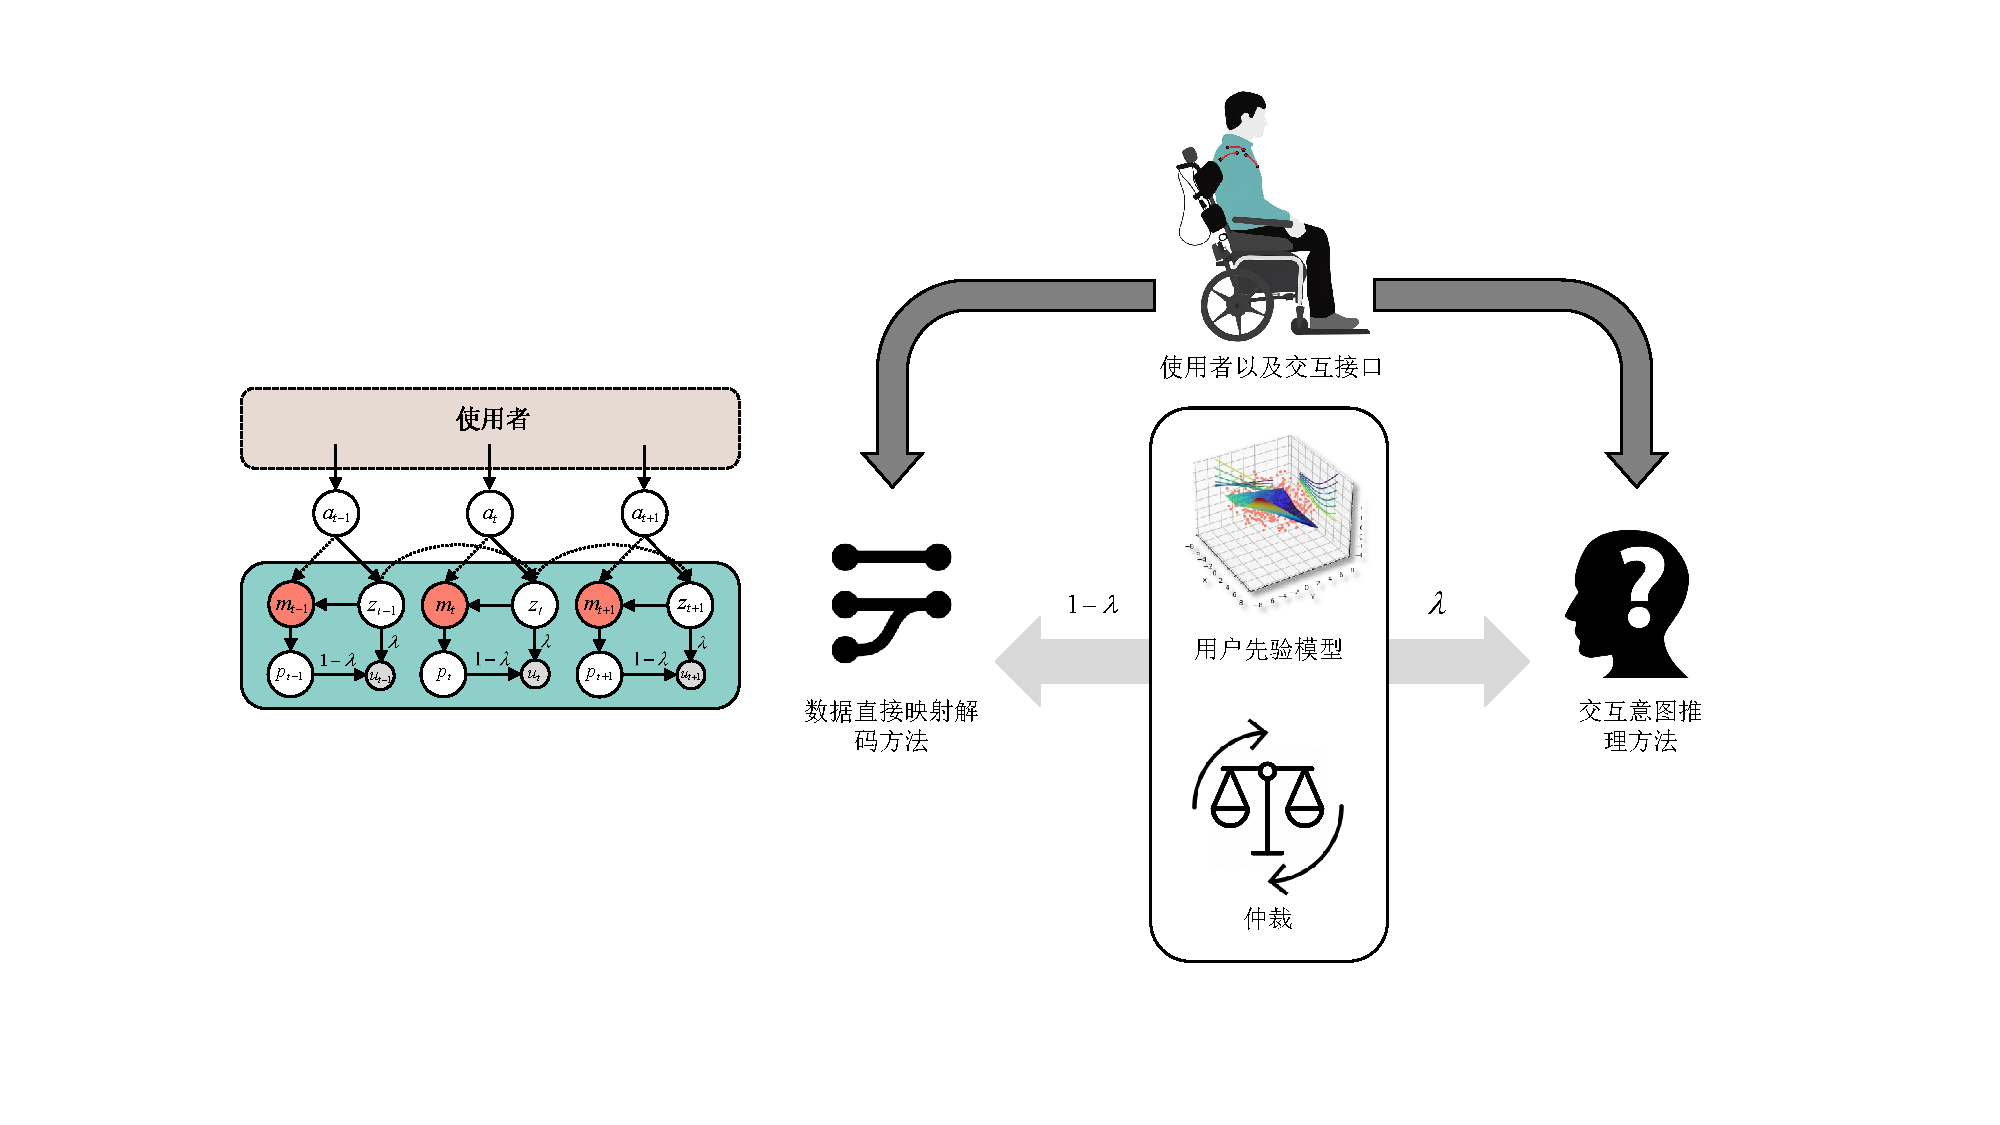
\includegraphics[width=1\textwidth]{figures/3-Fig-9.pdf}
    \caption{五名受试者的在感受野参数$r$由0.5至2.5设置下的用户能力模型热图}
    \label{fig:3-9}
\end{figure}  

共享自主系统用于切换解码方式的仲裁函数是基于一个由操控实验数据建模的非线性模型的,模型的感受野大小影响了指令解码切换的平滑度。图\ref{fig:3-9}给出了当感受野$r$从0.5增加到2.5时,五名参与者的能力模型的变化。通过选择合适的局部模型参数,可以实现泛化的$\mathcal{F}(u)$,从而在解码方式的切换过程中防止权重$\lambda_t$的突然变化导致的光标抖动。当$r=0.5$时,由于感受野过小因此无法建立可用的$\mathcal{F}(u)$,使其不适合用于共享自主的在线仲裁切换。随着感受野$r$半径的增加,模型泛化性能不断地提高,然而,过大的感受野可能会导致模型表现出过度平滑效果,导致其丢失局部特征。因此,在应用中需要平衡模型泛化性和保留局部特征这一,作为基准在本章中统一设置参数$r=2.2$。此外,实验观察到不同参与者的$\mathcal{F}(u)$表现出一些共同的特征。从图\ref{fig:3-9}中可以看出,五名实验参与者在命令空间中的第一象限通常表现最出色,但在第四象限表现最差。这可能是由于柔性体-机交互设备的设计缺陷所导致的,位于右肩的软传感器比左肩涉及更多的不确定性干扰,参与者在控制光标时遇到挑战。另外,在实验中观察到,与第一和第二象限相比,参与者在第三和第四象限的表现较差。这一观察结果与肩部运动的直观本质相一致,参与者表示控制肩部向前移动通常比向后移动更容易进行对光标的精确控制。  

\section{实验流程与设置}基于所设计交互界面和数据解码方法,研究通过一系列操作任务实验来评估不同解码方法的表现。9名健康受试者(年龄:$26\pm3$;性别:6男3女;身高:$174\pm16$cm;体重:$67\pm17$kg)参与了本研究并签署知情同意书。所有参与者在实验前都对所设计交互设备进行了为期2天的了解使用,以熟悉操作方法。在实验中要求所有受试者被要求将他们的小臂和手放在桌子上保持固定,以模拟上肢残疾的患者。

\subsection{标准目标到达实验任务流程}   
    \subsubsection{八方向目标到达任务}在这项任务中,参与者需要操作直径为0.8厘米的蓝色光标,将其移动到八个固定、预先设置的目标上。这些目标直径为2.4厘米,均匀分布在直径为26厘米的圆周上,两两之间相隔45度。任务起始时,用户需将光标对准位于指令空间中央的中心目标。接着,最右侧的目标首先激活,其余目标将按逆时针方向依次点亮。用户必须将光标在每个目标上稳定保持2秒以上才算完成该环节。如果12秒内未能完成环节,系统会自动跳转到下一个目标,并将未完成的环节记录为失败。

   \subsubsection{随机目标到达任务}在该任务中,实验在直径为26厘米的圆上均匀生成8个随机目标点。此任务类似于“八方向目标到达任务”,要求用户将光标导航至随机出现的目标区域,任务完成后再将光标返回至起始点。

\subsection{实验一:不同传感器配置模式用于意图推理的消融对比实验} 多模态方法在提升物体信息获取准确性方面已受到广泛的认可和应用,例如医疗决策辅助系统和组合导航系统\cite{williamsonContinuousUncertainInteraction2006}。此类方法可通过利用额外的模态数据为推断算法积累可以用于推断意图的证据。然而,目前尚未明确冗余的感知信息能否显著提升人机交互接口的性能。为了探究这一问题,我们在研究中设计了一项消融实验,旨在探讨各种传感器配置对意图推断过程的影响。表\ref{tab3-1}列出了六种预设的传感器配置。我们要求所有参与者针对每个传感器配置完成``八方向目标到达任务''五次,并在传感器配置发生改变时重新训练交互意图推理解码模块。为了减轻疲劳对实验结果的影响,在每项任务之间参与者拥有2分钟的休息时间。 

\begin{table}
    \centering
    \caption{用于意图推理的传感器数据源配置模式}
    \setlength{\tabcolsep}{3pt}
    \begin{tabular}{c p{180pt} c }
    \hline\hline
    配置模式代号 & 数据源使用 & $N$ \\ 
    \hline
    OS& 仅拉伸数据& 4 \\ 
    BS& 拉伸和弯曲数据&12 \\ 
    GS& 陀螺仪+拉伸数据&7 \\ 
    GBS& 陀螺仪+拉伸和弯曲数据&15 \\ 
    AGS& 加速度计+陀螺仪+拉伸数据&10 \\ 
    AGBS& 加速度计+陀螺仪+拉伸和弯曲数据&18 \\ 
    \hline\hline
    \end{tabular}
    \label{tab3-1}
\end{table}     

\subsection{实验二:目标到达任务中不同交互解码方法的比较} 每位参与者按顺序完成了八方向目标到达任务、虚拟动力轮椅驾驶任务和随机中心向外目标到达任务,每项任务均进行了五次。为确保任务结果的公正性,参与者未获知解码方法的具体技术细节,仅知道所使用方法的名称。为适应新的解码方法,在每次实验前参与者拥有2分钟的时间来熟悉在任务空间中的操作。此外,在进行电动轮椅驾驶任务之前,研究确保每位参与者通过使用设计的交互接口和标准的轮椅操纵杆来熟悉驾驶任务。参与者按以下顺序使用两种交互接口完成任务:操纵杆、基于确定性规则映射的命令解码、基于意图推理的命令解码以及共享自主切换的数据解码方法的柔性交互接口。每个参与者执行任务三次。 

\subsection{实验三:虚拟电动轮椅驾驶任务中不同交互解码方法的比较}电动轮椅作为一种移动辅助设备,是残疾人辅助器具中最为重要的一种。研究基于两轮差速移动机器人模型,设计了如图\ref{fig:3-13}(B)所示的虚拟电动轮椅驾驶场景。在该任务中,参与者需要在尽可能短的时间内驾驶虚拟轮椅穿越一系列障碍,其中的碰撞次数和任务完成时间被同步记录用于量化实验表现。

\section{实验与分析}

\subsection{交互效果评价量化指标}   
 \subsubsection{完成任务花费的时间(TS)}该指标涉及用户从任务空间中心移动光标至目标位置所需的持续时间。较短的移动时间反映了解码算法的准确性和效率的提高。
 \subsubsection{平均轨迹偏移距离 (AveOD)}该指标评估了光标相对于连接中心目标和激活目标之间直线路径的平均偏移量,用于反映光标在任务空间中移动的线性程度。较高的``AveOD''值表明光标经常偏离用户期望的路径,从而需要用户投入更多的精力来控制光标。
 \subsubsection{平均光标移动速度(AveSpeed)}该指标是根据用户控制光标的平均速度计算得出的。 “AveSpeed”值越高表示接口具有越高的动态性能。
 \subsubsection{平均光标运动急动度 (AveJerk) }该指标是通过计算用户在任务空间中控制的光标位置相对于时间的三阶导数来确定的。较高的``AveJerk''值表明用户对光标的控制不够平滑,并且存在较多抖动。在这种情况下,``抖动''指的是光标发生的不可预测的小而快速的移动。  

\subsection{最优传感器配置模式}图\ref{fig:3-10}(A)为使用柔性体-机交互接口的参与者在不同传感器配置下执行实验任务的表现量化指标的分布情况。图\ref{fig:3-10}(B)显示了被控制光标在任务空间中一些典型的运动轨迹。本章节中的数据分析基于单因素方差分析方法(one-way ANOVA)进行统计显著性检验。实验数据表明,与OS配置模式相比,使用BS传感器配置方法的操控表现提高并不显著。尽管将柔性传感器的弯曲数据用于交互意图推理并相较于OS模式在一定程度上改善了动态性能(平均``AveSpeed''从0.141m/s增加到0.149m/s),但也导致了操控线性度的下降(平均``MaxOD''从2.06cm上升至2.28cm)。这一发现表明,使用柔性传感器的弯曲信息可能会在交互意图的推理中引入更多的不确定性因素,这是因为某些软传感器在肩部运动期间可能会使得交互接口在无意中向不可预测的方向弯曲导致的。在GS模式中,陀螺仪数据的加入显著提高了任务的完成效率($p<0.001$)。与仅使用柔性传感器拉伸信息的OS模式相比,GS模式具有较低的``TS''表现(平均2.11秒)和较高的``AveSpeed''表现(平均0.16 m/s)。此外,使用GS配置模式还降低了``TS''和``MaxOD''指标的标准差,并且光标移动的轨迹表现出相较于其他模式更好的线性度。这主要归功于陀螺仪的具有较高的动态性能表现,此外陀螺仪仅检测使用者上半身的整体相对运动,而不是肌肉活动,因此减少了穿戴式交互接口中不确定性因素的影响。使用了三种传感器信息的GBS配置模式并没有显著提高意图推理控制光标的性能。相反,与之前分析的原因类似,虽然与``GS''模式相比,它在一定程度上提高了``AveSpeed''的表现($p<0.01$)。但是其仍然会导致任务完成效率和平滑度表现变差,体现在GBS模式拥有较高的``TS''($p<0.001$)和``AveJerk''($p<0.001$)值。

\begin{figure}[htb]
    \centering
    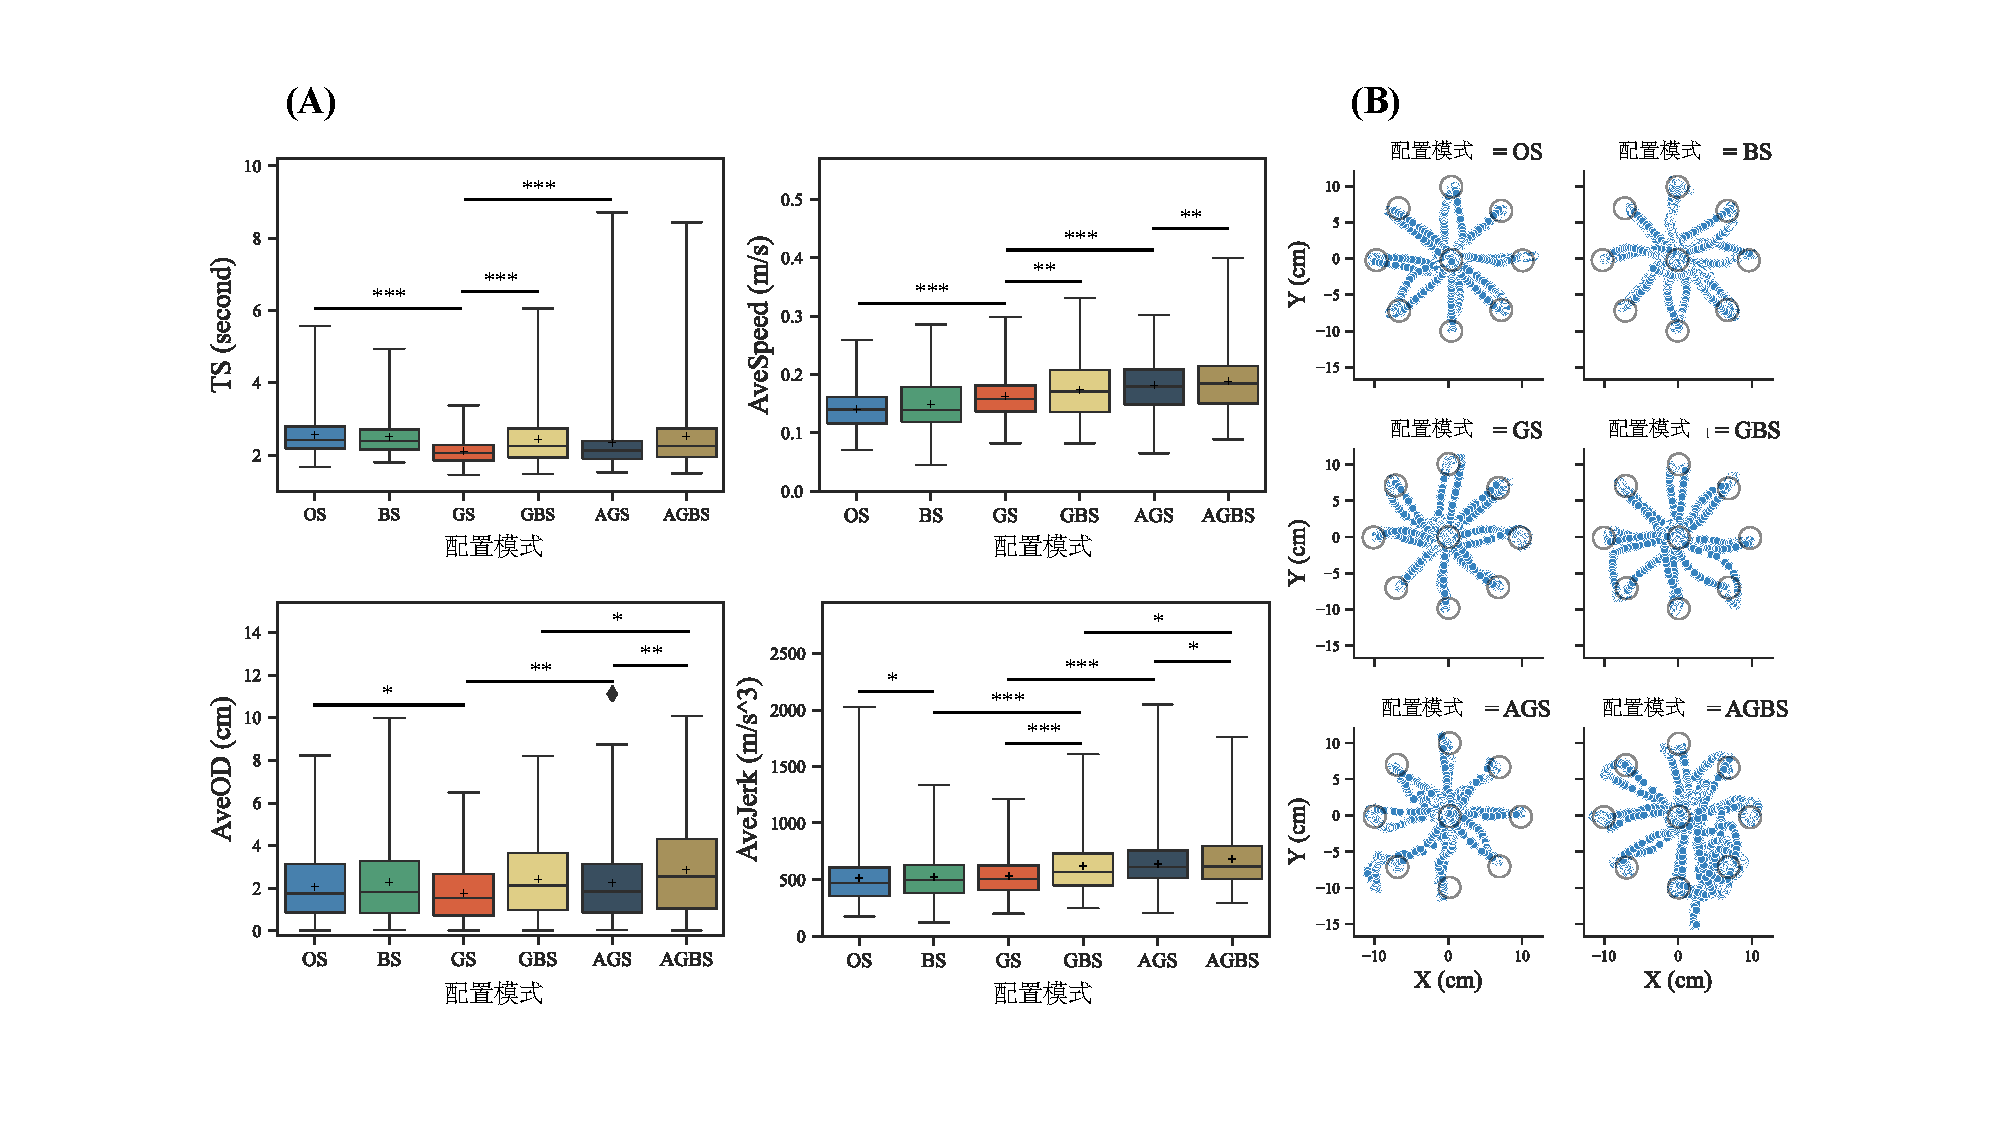
\includegraphics[width=1\textwidth]{figures/3-Fig-10.pdf}
    \caption{(A) 最佳传感器配置实验中不同配置的性能, 其中``*''代表$p<0.05$,``**''代表$p<0.01$,``***''代表$p<0.001$。 (B) 不同传感器配置下``八方向中心向外目标到达任务''的任务空间轨迹。}
    \label{fig:3-10}
\end{figure}  
加速度计的使用可最大化所有配置中``AveSpeed''的值(其中AGS配置模式为 0.181 m/s,AGBS模式为0.188 m/s),但是其同样也会增加时间花费``TS''的方差。与没有使用加速度计进行意图推理的GS和GBS配置模式相比,AGS和 AGBS模式的线性度和平滑度相对较差,体现在他们具有明显更高的``MaxOD''($p<0.01$)和``AveJerk''($p<0.05$)。如图\ref{fig:3-10}(B)所示,研究发现AGS和AGBS模式中的光标轨迹明显比其他配置模式更加不规则,这是因为实验参与者在操控任务空间中的某些区域无法很好地控制光标,导致需要频繁修正光标的位置所导致的。此外,研究发现在使用意图推理进行光标操控时,当不使用加速度计时所有参与者都在指定的时间内成功完成了目标到达任务。然而,我们观察到一些参与者在实验中无法使用AGS和AGBS配置完成任务。之所以会出现这个问题,是因为加速度计作为一种绝对量传感器,对用户的上半身的绝对姿态较为敏感。因为我们假设了用户的意图与交互接口的传感器测量之间存在线性关系,即使使用者身体姿势的微小调整也会对意图推断产生重大影响。它会导致生成的命令经常偏离用户的意图,使参与者难以保持对光标的控制。

综合来看,消融实验的结果表明仅使用陀螺仪角速度信息和柔性传感器拉伸信息的GS配置模式表现出最综合的性能优势,其具有更为优异的任务完成效率和线性度,同时保持了对光标操控的动态性能。因此,在本研究中选择了仅包含陀螺仪和柔性传感器拉伸信息GS模式作为意图推理的基准配置。

\subsection{三种解码方法的实验表现与分析}     
\subsubsection{八方向目标到达任务实验表现}图\ref{fig:3-11}(A)显示了前文中所提到的三种不同数据解码方法在八方向目标到达任务中的实验表现。相较于其他两种解码方式,尽管基于确定性规则直接映射解码模式(DCM)在``AveSpeed''($p<0.001$)指标方面具有优势,但与意图推理模式(UII)相比并没有显著改变任务完成时间花费指标``TS''。这是因为使用直接映射解码的参与者经常超越任务目标的中心位置,因此参与者往往需要更多的时间来调整操控光标,使其保持在激活的环形目标的范围之内导致降低了任务完成效率。此外,在实验中我们发现由于柔性传感器的在使用者运动中的不确定性形变常常会导致光标向使用者意想不到的方向移动。然而,交互设备使用者通常能够借助显示屏的视觉反馈快速调整光标的位置,但这会在一定程度上增加他们的认知负担。  
\begin{figure}[htb]
    \centering
    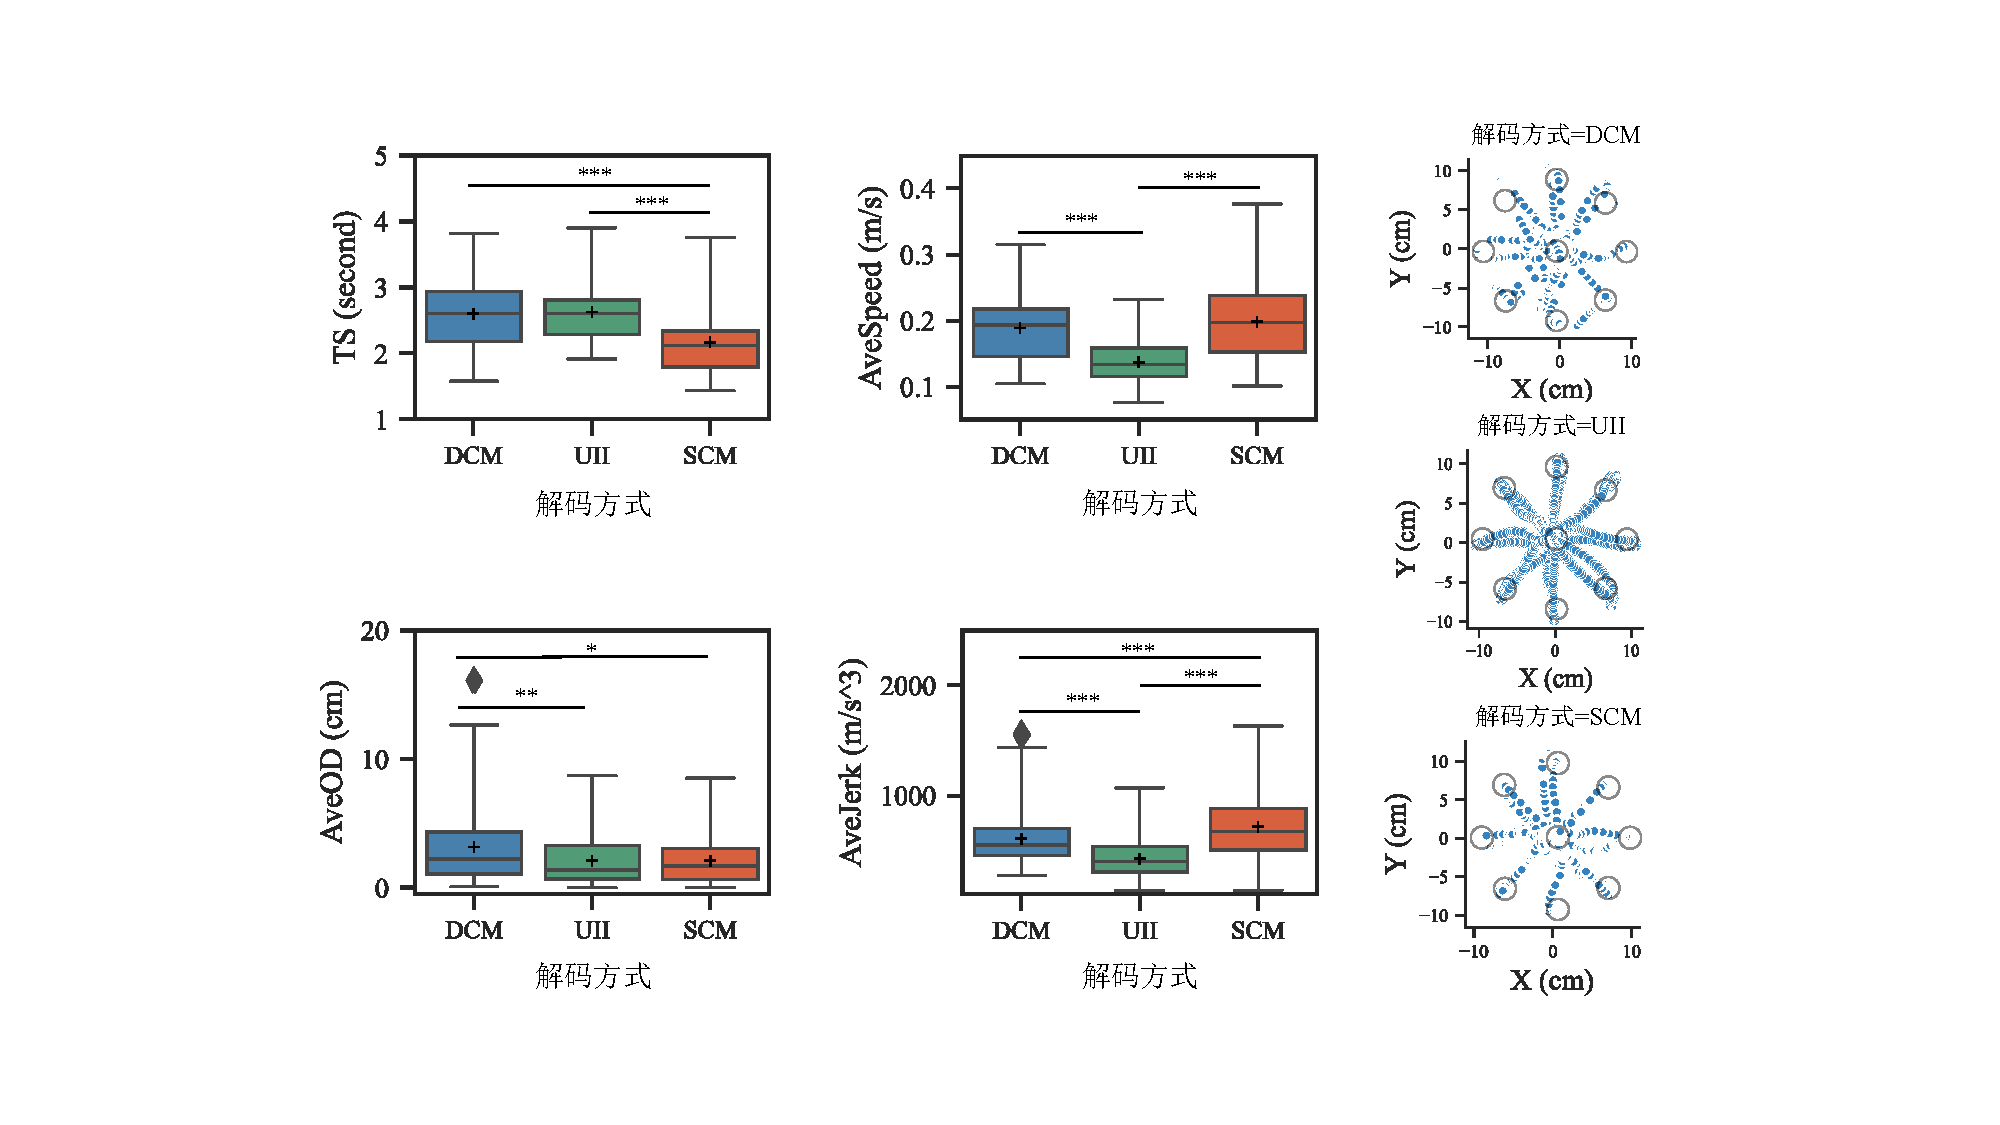
\includegraphics[width=0.7\textwidth]{figures/3-Fig-11.pdf}
    \caption{不同解码方法在完成``八方向中心向外目标到达任务''中的表现性能指标,其中“*”代表$p<0.05$,“**”代表$p<0.01$,“***”代表$p<0.001$,以及使用不同解码方法完成任务的光标运动轨迹。}
    \label{fig:3-11}
\end{figure}     
   
意图推理需要更多的来自传感器的证据积累,这导致其与直接的数据映射动态性能的下降。尽管存在这一缺点,意图推理方法在光标移动线性度``AveOD''($p<0.01$)和平滑度``AveJerk''($p<0.001$)方面表现出了显著的优势。与DCM模式相比,从其较低的``AveOD''和``AveJerk''值可以明显看出这一点。 基于意图推理的方法的光标操控运动轨迹通常更直接地到达目标,需要参与者较少的实时纠正和调整。这表明意图推理方法在控制光标方面提供了更好的准确性和精度。与基于规则的直接数据映射方式相比,意图推理虽然显著降低了``AveSpeed''的值,但提高了任务完成的效率,这从两种方法之间相似的“TS”性能中可以明显看出(在更低的平均速度下,拥有相似的任务完成效率)。意图推理的这一特性通过最大限度地减少光标操作过程中对于控制结果反馈校正或微调的需要,增强了整体用户体验。

基于共享自主的自适应解码方案(SCM)与DCM模式具有类似的``AveSpeed''性能表现,但是显著降低了实验中的``TS''值($p<0.001$),这表明使用SCM模式相较于DCM模式具有更好的任务完成效率。此外,SCM模式和UII模式在光标操控线性度指标``AveOD''上具有相似的性能,但是其明显优于DCM模式($p<0.05$)。这表明,SCM在一定程度上结合了DCM的高动态特性和UII的高精度特性。在实验任务中,实验参与者表示在使用自适应解码方案时可以清晰地感受到意图推理辅助的干预。在用户使用DCM模式表现良好的区域,SCM使得用户主要使用DCM来控制光标因此保证了操控的高动态性能。反之,在参与者使用DCM模式表现不佳的区域,共享自主解码方式将操控模式无缝切换至意图推理,通过降低一定的动态性能进而保证光标控制的准确性。然而,在自适应切换过程中也带来了一个问题,即被控制的光标由于仲裁函数的对于解码方式的动态调整而容易产生一些抖动。因为与DCM和UII模式相比,SCM模式具有明显更高的``AveJerk''值($p<0.001$)。

\subsubsection{随机目标到达任务实验表现}在具有固定目标位置的八方向目标到达任务的基础上,研究进一步测试了使用者使用三种解码方法在任务空间不同区域到达随机目标的表现情况。图\ref{fig:3-12}给出了一位参与者的任务空间中的一些代表性光标轨迹。与具有更高``AveSpeed''值的UII模式相比,参与者使用DCM模式通常需要更多时间($p<0.01$)来完成任务。SCM显示出明显低于 DCM 和 UII 的任务花费``TS'',表明其相较于其他两种解码模式显著提升了任务的完成效率($p<0.001$)。 基于意图推理的方法仍然具有最好的线性度和平滑度,表现在其仍然具有最低的``AveOD''和``AveJerk''值。如图\ref{fig:3-12}所示,研究进一步分析了参与者使用SCM解码方式控制光标分别达到位于象限I/II和象限III/IV的目标的表现。在任务空间的象限I/II 中,SCM与DCM模式具有相似的性能。在象限 III/IV 中,尽管会引起一些抖动,SCM模式相较于UII模式在明显提高了平均速度``AveSpeed''的基础上($p<0.05$),同时保持与UII类似的操控线性度指标``AveOD''。综合来看,SCM模式通过将预实验中用户使用DCM模式的表现先验知识纳入一个共享自主自适应框架中,实现了由动态性能较高的直接数据映射到更加准确平滑的意图推断解码的无缝切换,在保证了操控动态性能的前提下确保了生成命令的准确性。  

\begin{figure}[htb]
    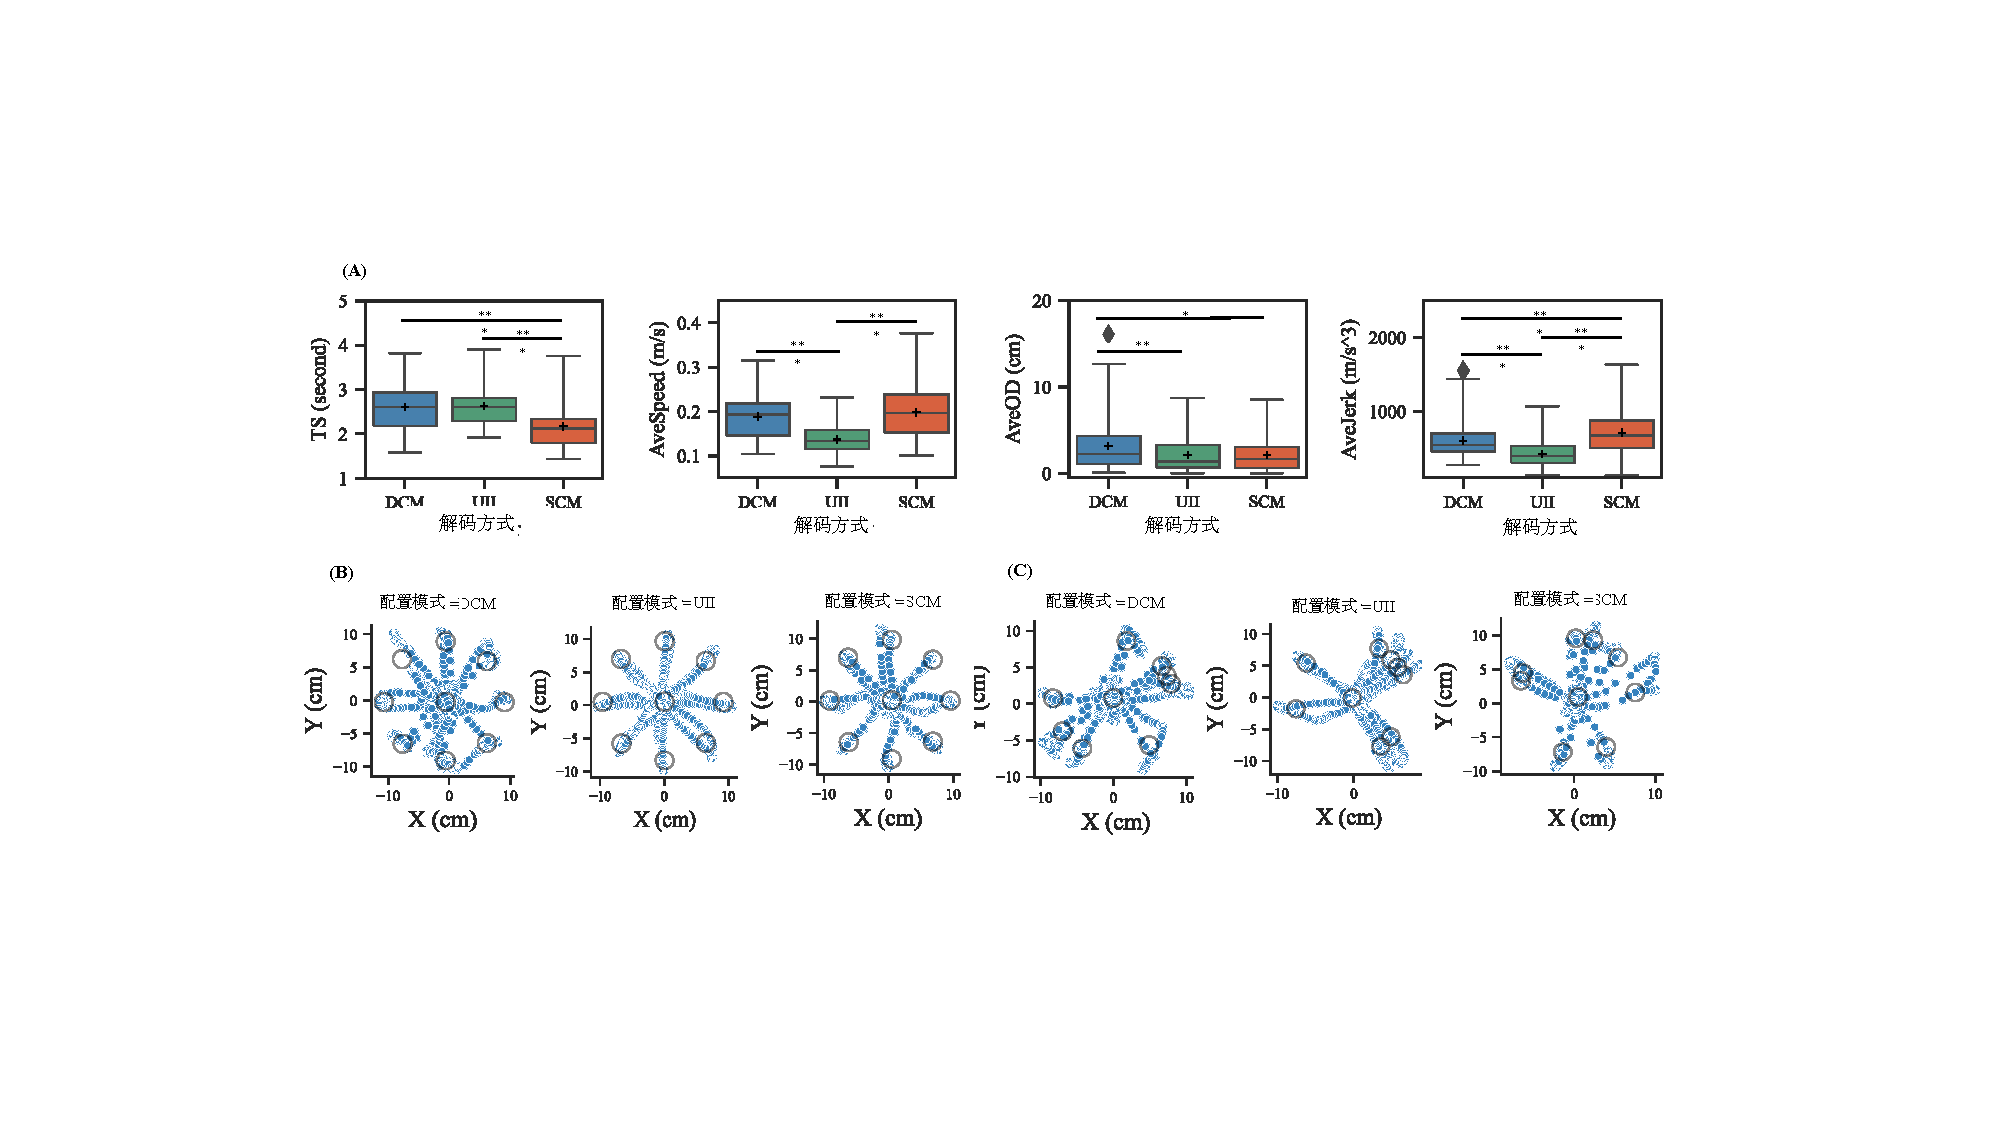
\includegraphics[width=1\textwidth]{figures/3-Fig-12.pdf}
    \caption{(A)“随机中心向外目标到达任务”中不同解码方法的轨迹。 (B) “随机中心向外目标到达任务”的象限 I/II 和 III/IV 中的表现,其中“*”代表$p<0.05$,“**”代表$p<0.01$,“***”代表$p<0.001$。}
    \label{fig:3-12}
\end{figure}

\subsubsection{虚拟电动轮椅驾驶任务实验表现}     
  
\begin{figure}[htb]
    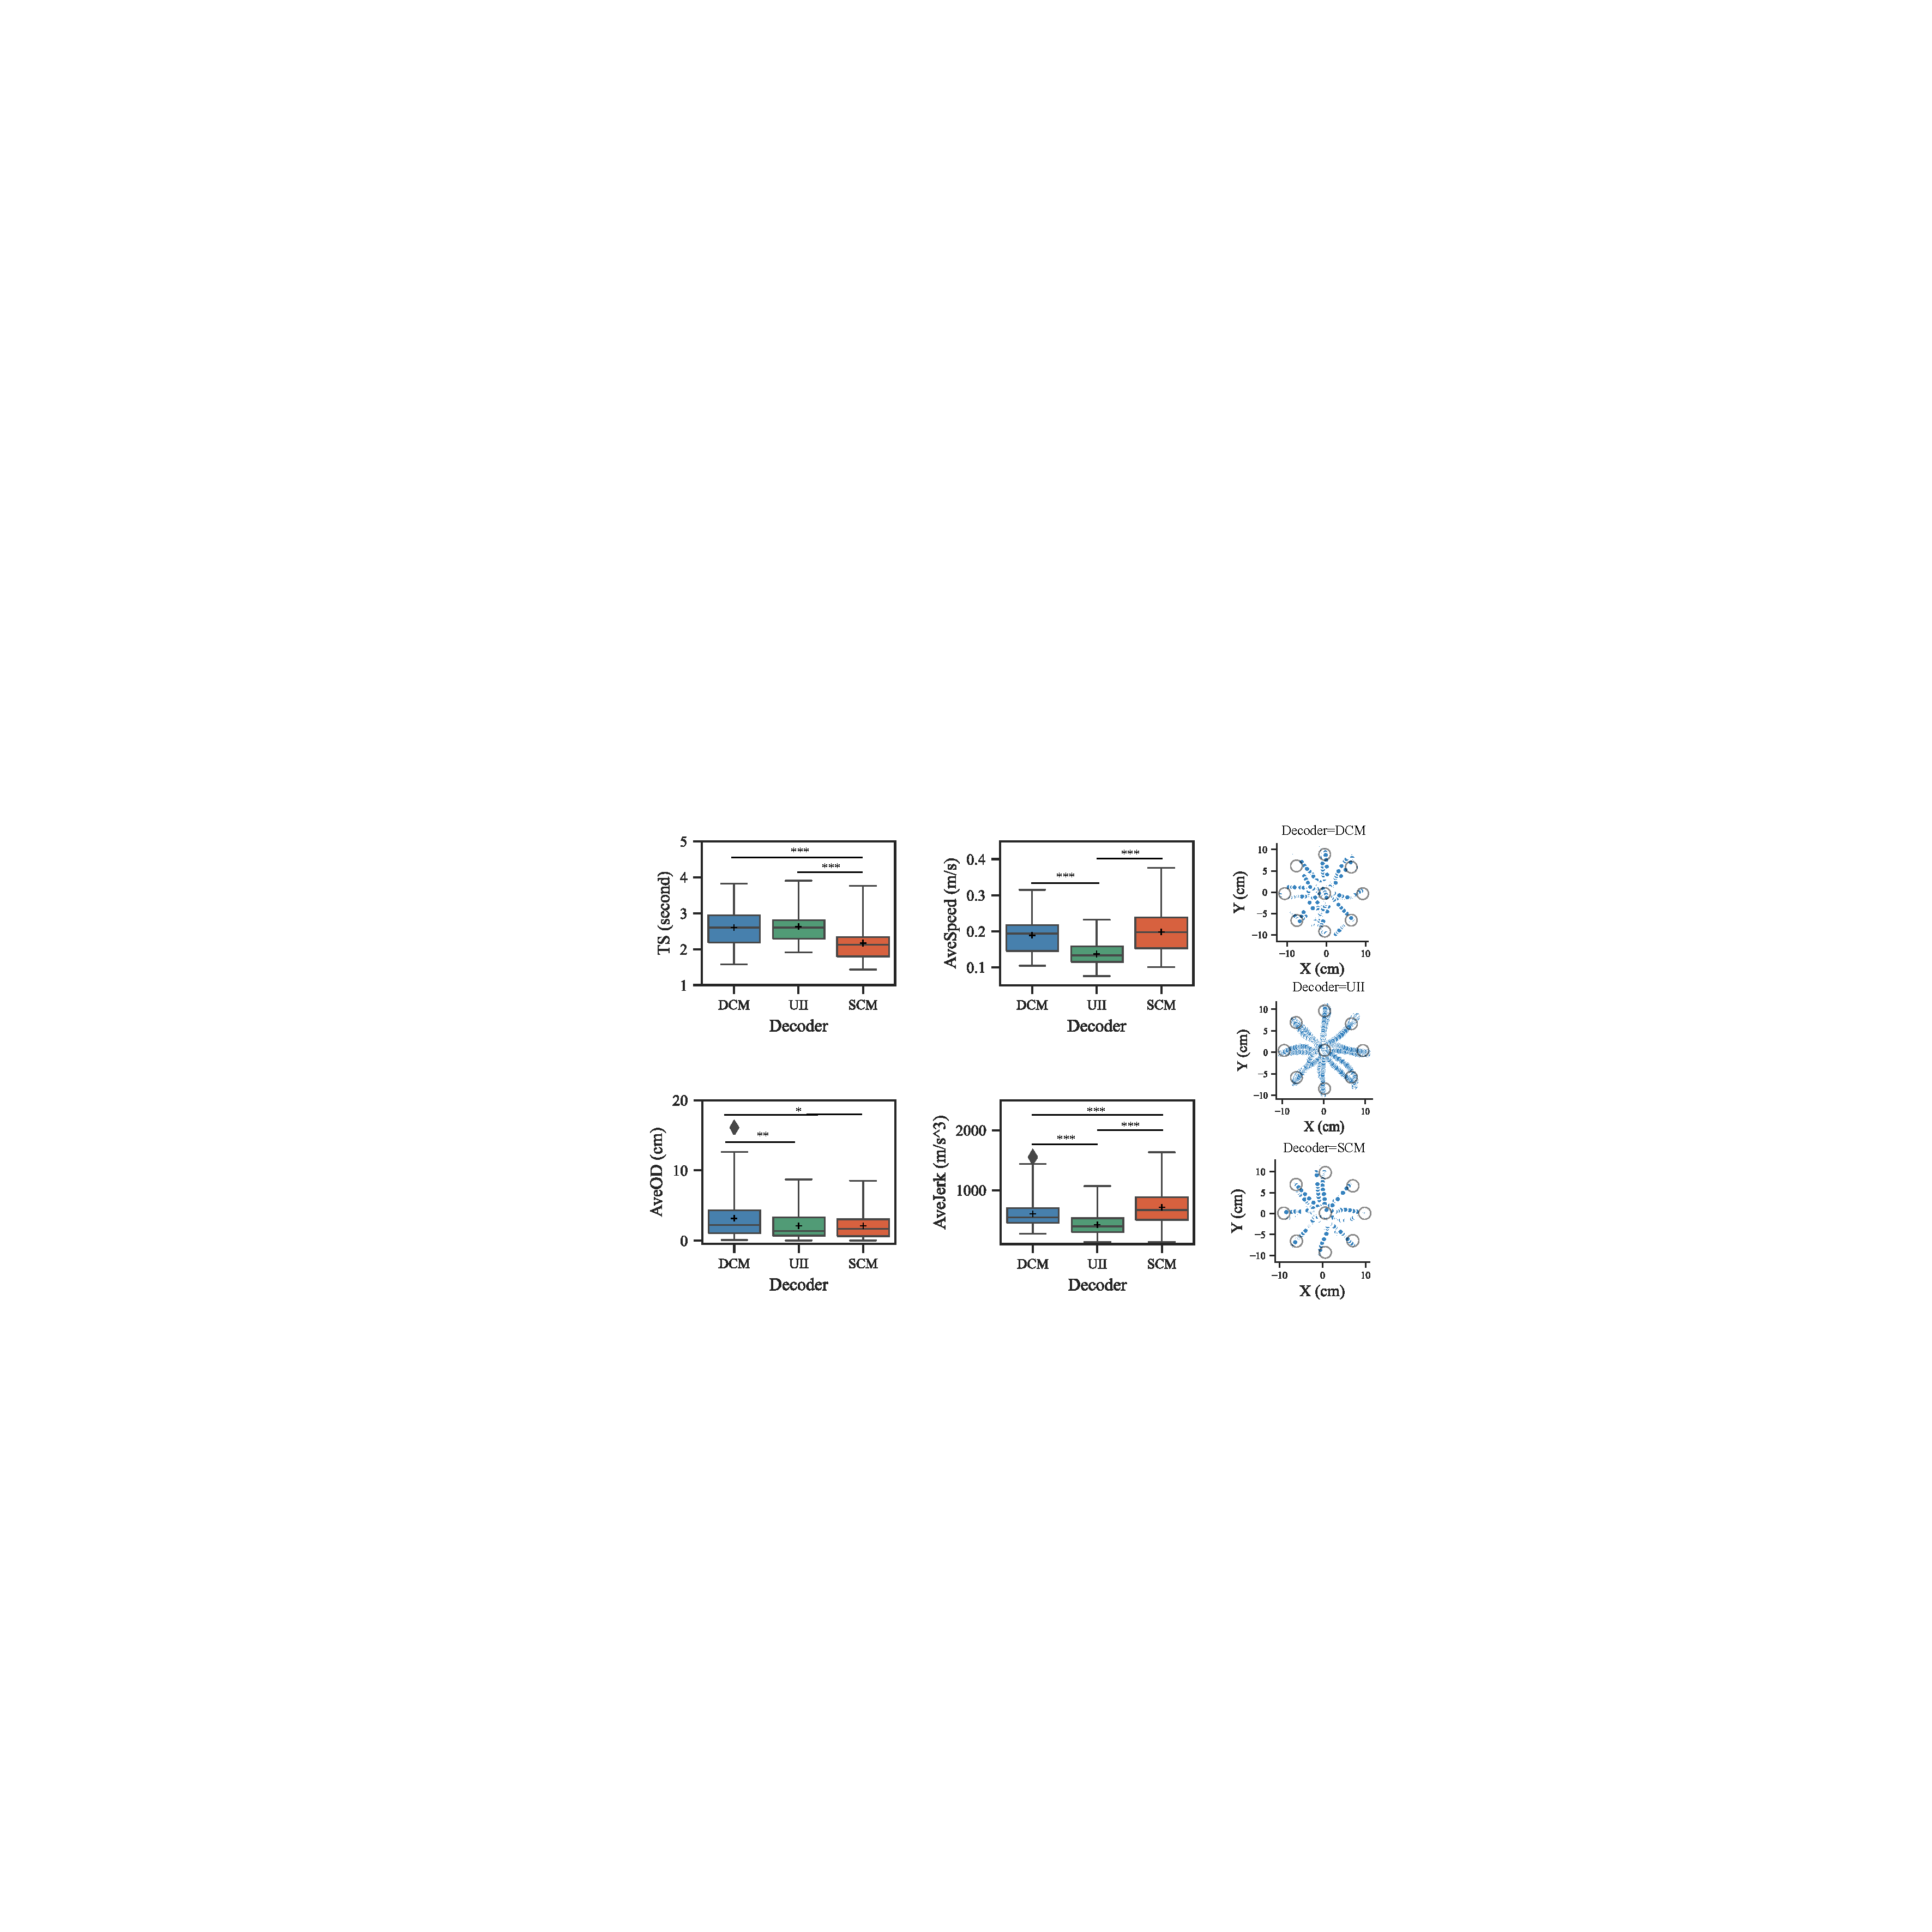
\includegraphics[width=1\textwidth]{figures/3-Fig-13.pdf}
    \caption{(A) 由轮椅操纵杆和所开发柔性人机交互接口在不同解码方式下操控虚拟电动轮椅完成任务的运动轨迹,其中红色标记表示发生碰撞。(B) 虚拟电动轮椅驾驶场景的 3D 渲染。 (C) 在轮椅驾驶任务的命令空间中生成命令,其中蓝色区域是死区。}
    \label{fig:3-13}
\end{figure}  

图\ref{fig:3-13}(A)显示了参与者使用操纵杆和不同解码模式下的柔性-体机交互设备操控轮椅在虚拟场景中的运动轨迹。表\ref{tab3-2}总结了虚拟轮椅操控的实验表现,当使用操纵杆时参与者完成任务的时间通常较短,平均为29.63秒,并且遇到的平均碰撞次数最少,约为3.4次。操纵杆良好的触觉反馈有助于平稳、精确地控制虚拟轮椅,使参与者能够沿直线操纵它并轻松进行微调。 当使用所开发的体-机交互接口时,采用DCM解码方式的任务平均完成时间与使用操纵杆类似,但其控制精度较低,容易在狭窄空间内发生碰撞因此平均碰撞次数相较于操纵杆更高。  

\begin{table}[htb]
 \centering
 \caption{虚拟电动轮椅操控实验表现}
 \setlength{\tabcolsep}{5pt}
 \begin{tabular}{c c c}
 \hline\hline
  交互方式 & 任务完成花费时间 & 碰撞次数  \\  
 \hline
 轮椅操纵杆&     $29.63\pm 2.23$      s&        $3.4$         \\ 
 柔性交互接口+DCM解码&        $31.46\pm 2.26$        s&        $15.8$         \\ 
 柔性交互接口+UII解码&        $35.38\pm 1.63$        s&        $61.8$         \\ 
 柔性交互接口+SCM解码&        $31.12\pm 1.03$        s&        $11.6$         \\  
 \hline\hline
 \end{tabular}
 \label{tab3-2}
\end{table}     

参与者在使用UII解码方式时表现最差:在该模式下的完成任务时间最长,并且在移动中经历了更多的碰撞。如图\ref{fig:3-13}(A)所示,在任务开始时的直线行驶过程中,UII的轮椅轨迹有明显更高的振幅振荡。这是因为UII显著增加了整个闭环控制系统的延迟。大多数参与者需要很长的调整时间才能稳定对轮椅的控制。这是由于意图推理存在较高的延迟,使用者必须隐式地建立对肩部运动和交互接口动态的内在信念,但在复杂的肩部运动中实现这一点可能具有挑战性使得在交互操控中出现震荡。  

另外,我们观察到SCM模式和DCM模式在轮椅操控中的表现是相似的。与意图推理方法相比,这两种方法在闭环系统的动态性能方面都表现出了显著的优势。这是因为设计的虚拟场景不存在需要大曲率转向的弯道区域,因此交互过程中产生的命令主要集中在命令空间的第一象限和第二象限(如图\ref{fig:3-13}(C)所示)。正如上一小节所讨论的,SCM模式在这些区域中将自动切换为以DCM为主的解码方式进行操控,因此SCM模式与DCM模式具有类似的操控体验。尽管如此,某由于仲裁切换引起的抖动可能仍然会影响虚拟轮椅的控制精度,这从SCM比 DCM 发生更多的平均碰撞次数可以看出。  

实验表明,人机交互系统的控制效果不仅取决于用户对观察状态与预期状态的比较,也与被控系统的响应速度相关。在动作与系统响应的延迟较短情况下,比如使用DCM和SCM系统,用户可以通过内部建立一个简单的比较器控制器来实现稳定控制,这时系统延迟被隐式视作一个常数;而在延迟较长的场景下,用户则需要建立较为复杂的预测模型,这要求参与者花费更多时间去适应和学习。例如,我们观察到参与者在使用意图推理解码时,控制模式常从连续过渡到基于短信号的突发式控制。同时,微小的偏差可能会引起参与者过度反应,造成对轮椅控制的失稳。为了避免碰撞,实验中参与者往往降低行驶速度以达到稳定控制,这也导致UII模式下的任务平均完成时间最长。

\subsection{用户研究:在目标到达任务中参与者表示更喜欢基于共享自主系统的自适应切换解码方法}在目标到达任务中,七名参与者表示相对于DCM和UII更喜欢SCM模式,理由是其具有较好动态性能和光标操控准确性。参与者表示在使用DCM模式时,光标经常偏离到非预期位置,尤其是在命令空间的第三和第四象限中,而此问题在第一和第二象限中出现的频率较低。它导致 SoftBoMI 对于参与者来说变得``不可预测''。然而,当任务完成时间不是优先考虑的时候,参与者可能会优先选择UII模式,因为它提供更流畅、更准确的交互意图解码。  

\subsection{用户研究:在虚拟电动轮椅驾驶任务中,参与者更喜欢直接规则映射和基于共享自主自适应切换的解码方法而不是意图推理}在虚拟电动轮椅驾驶任务中,五位参与者表示偏好DCM模式,四位参与者偏好SCM模式,没有受试者偏好UII模式。七名受试者表示,他们没有意识到DCM和SCM模式之间存显著差异。大部分参与者表示,基于意图推理的UII模式存在的高延迟使得他们难以快速稳定地控制虚拟轮椅。

\section{本章小结}本章节介绍了一种集成多个柔性弯曲拉伸传感器及一个惯性传感器的新型非侵入式可穿戴体-机交互接口设计。该接口能将肩部残余运动映射到二维连续控制空间。上半身运动由IMU捕捉,特定肌肉活动则由软传感器检测,以此提升交互设备的动态性能和可靠性。研究中采用概率图模型分析人机交互中的不确定性,设计了基于规则的确定性数据映射解码方法,及针对肩部动作不确定性的意图推理数据解码方法。另外,还提出了基于共享自主系统的自适应切换解码方法,集成先验表现到非线性仲裁函数中,实现了确定性数据映射与用户界面交互的平滑过渡。实验结果显示,该方法可提高命令生成的准确性,确保适应不同任务的动态性能。然而当前工作仍然存在局限,如在意图推理中采用线性状态转移和高斯先验的简化假设,不一定适用于高维命令空间。另外,用户交互主要依赖视觉反馈,缺少本体感觉。为提升可用性,未来可考虑将其他反馈机制集成到交互接口设计中。
